\chapter{Modelling object lifetimes in finite networks under churn}
\label{chp:MODELLING}

The purpose of this chapter is twofold: to validate the expected object lifetimes measured using the Oversim simulation of Pithos and to provide a tool for designing distributed storage systems with expected object lifetimes. This is done by developing a statistical model for object lifetimes, which is used to verify the simulation results.

During the Pithos evaluation, it was found that user groups can be limited in size, in that the average group size is comparable to the number of required replicas. Object lifetime prediction models were found in the literature that assume an infinite network size, but none that take into account the network size.

\section{Background and related work}
\label{model_related_work}

To increase the time an object is available within a distributed storage system, two techniques are used: redundancy and repair. In storage systems using replication as redundancy technique, $R$ replicas of every object are stored. The number of required replicas $R$ is a design decision, the effect of which will be shown in Section \ref{results}. When all nodes containing an object's replicas have left the network, the object is no longer available. Periodic repair, which occurs at a rate of $\mu = 1/T_{\textrm{repair}}$, replaces all missing replicas.

This chapter mainly extends and improves upon the work by Wu, Tian and Ng \cite{replication_article}. The related work models three characteristics of distributed hash table (DHT) lookups under churn: expected lookup latency of various routing schemes, expected lookup overhead of various routing schemes and expected object lifetime. We focus on the object lifetime characteristic. Wu, Tian and Ng develop two models for object lifetime when exponentially distributed node lifetimes are assumed. One for the case without object repair and one for the case with object repair. Node residual lifetimes are used when calculating expected object lifetimes without repair. In this case object lifetimes are equal to the maximum residual lifetime of the nodes the objects were replicated on.

%What about Pareto lifetimes?

A continuous time Markov chain, shown in Figure \ref{fig_other_markov_chain}, is used to model the expected object lifetimes for the case with repair.
%
\begin{figure}[htbp]
 \centering
 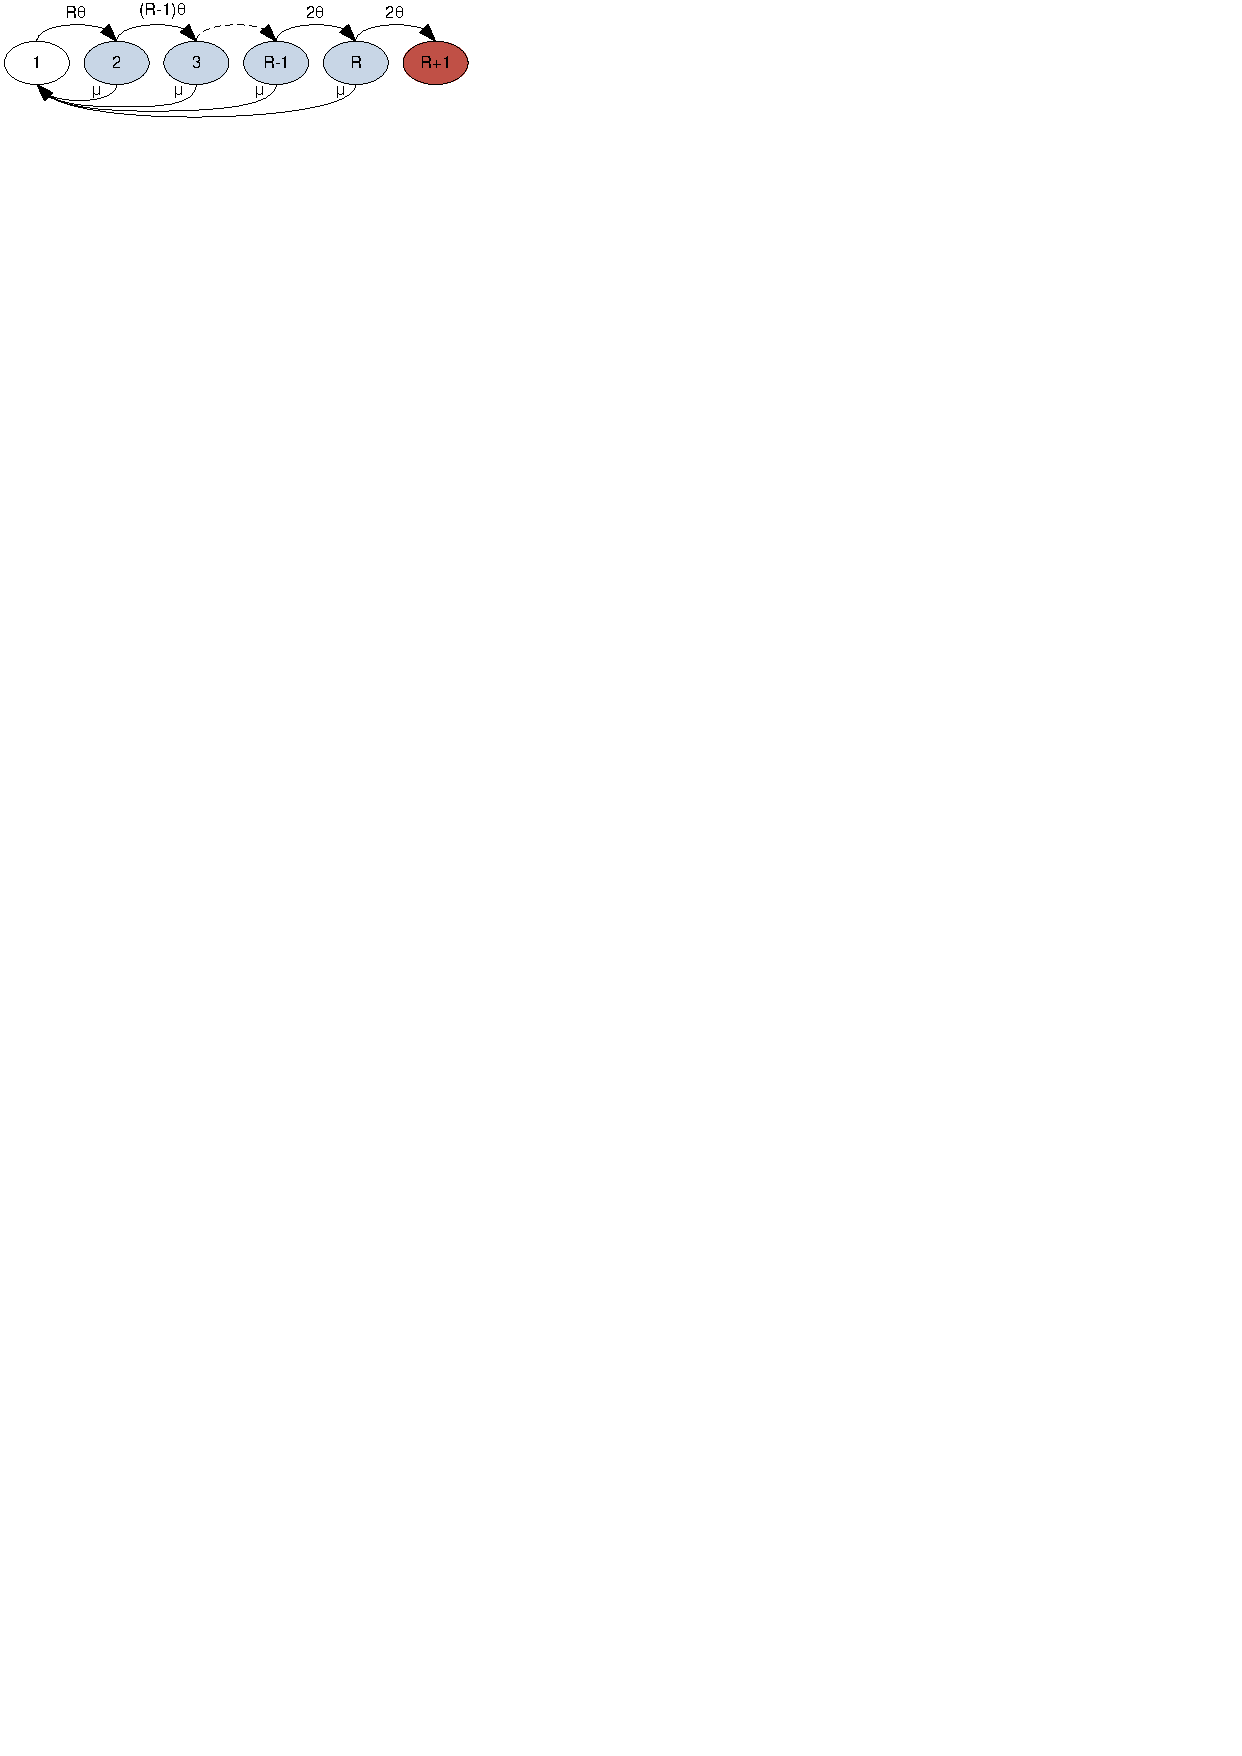
\includegraphics[clip=true, viewport=0.0cm 27.5cm 8.0cm 30.0cm, width=0.7\columnwidth]{inifinite_network_chain}
 \caption{Markov chain modeling object replica number for an infinite network size with repair.}
 \label{fig_other_markov_chain}
\end{figure}
%
The model has $R+1$ states and is in state $k$ when $R+1-k$ replicas are alive in the network. The system is, therefore, in state $1$ when all replicas are present and in state $R+1$ when no replicas are present. The authors assume that all objects are inserted into the network with $R$ replicas, i.e. enter the network in state 1. This initial state is colored white in Figure \ref{fig_other_markov_chain}. If the node departure rate (the rate at which nodes leave the network) under steady state is $\theta$ and there are $r$ replicas present in the network, the replica departure rate under steady state is $r\theta$. When all replicas are lost, the chain enters state $R+1$ (coloured dark) and is said to be ``absorbed''. This means it cannot return to any of the other states in the Markov chain.

In this chapter, we improve on the work by Wu, Tian and Ng \cite{replication_article} in two ways: firstly, the model is extended to take into account a finite network size, since there might not be sufficient nodes to replicate the data on when objects are stored or when the repair mechanism activates. Secondly, our model unifies the cases ``with repair'' and ``without repair'', to produce a single model where the effects of both might be evaluated. When our model is used with larger average network sizes, expected object lifetimes converge to those shown in the work by Wu, Tian and Ng, \emph{using their two separate models}.

Predicting object lifetimes in a distributed storage system is grounded in reliability engineering theory. When network size is ignored, it is similar to predicting the mean time to failure (MTTF) of a set of parallel components with repair. Chun et al. \cite{Chun:2006_replica_maintenance} also uses a Markov chain to model object replicas with network churn and repair. They use a birth-death process similar to the model by Wu, Tian and Ng, but using incremental, instead of complete repair.

No literature could be found in general reliability engineering or distributed systems reliability research that deals with object lifetimes with finite network sizes.

In the rest of the chapter we first show how the model of Wu, Tian and Nig was extended. We specifically discuss how expected object lifetimes can be calculated from our extended model. We use the results of these calculations to compare the simulated results of Pithos and validate the correctness (at least for object lifetimes) of the simulation.

\section{The model}
\label{model}

In order to model the effects of a finite network size on the lifetime of an object, the continuous time Markov chain model introduced in Section \ref{model_related_work} is expanded by adding a second parameter to every state, namely the network size. This effectively adds another dimension to the Markov chain. We also introduce $\phi$ to be the rate of arrival of nodes under steady state conditions.

Every state is a tuple of the form \verb.(replicas,nodes).. The state $(r, n)$ represents that $r$ replicas of an object are currently stored in a network currently containing $n$ nodes. $R$ is the required number of object replicas and $N$ is the maximum number of nodes in the network. It is assumed that $R$ replicas are always stored in the network, if sufficient space is available. If the number of nodes currently in the network $n$ are fewer than the required number of replicas ($n < R$), only $n$ replicas are stored. The initial states of the Markov chain are therefore all the states ($R,n$) as well as all the states ($n,n$), for $n < R$. There are therefore $N$ initial states, one for every possible network size. The initial state is the initial network size that an object is placed in.

If there are no more replicas in the network, an object cannot be repaired and the Markov chains remains in the set of states ($0,n$). These are said to be the absorbing states of the Markov chain and there exists $N - R + 1$ absorbing states in the model presented here. All other states out of which transition is possible are said to be transient states. It can be shown that if sets of transient and absorbing states exist, the system will always end up in the absorbing states \cite{grinstead1997introduction_probability}. The time to absorbtion can be calculated, which in the case of object storage means the time when no more objects exist in the network.

\subsection{State transitions}

There are four types of state transitions possible in the Markov model presented here:
%
\begin{enumerate}
\item A node that contains a replica departs the network.
\item A node that does not contain a replica departs the network.
\item A node joins the network.
\item An object is repaired.
\end{enumerate}

%In a continous Markov chain we define delta small enough so only one event can occur at any point in time

\begin{figure}[htbp]
 \centering
 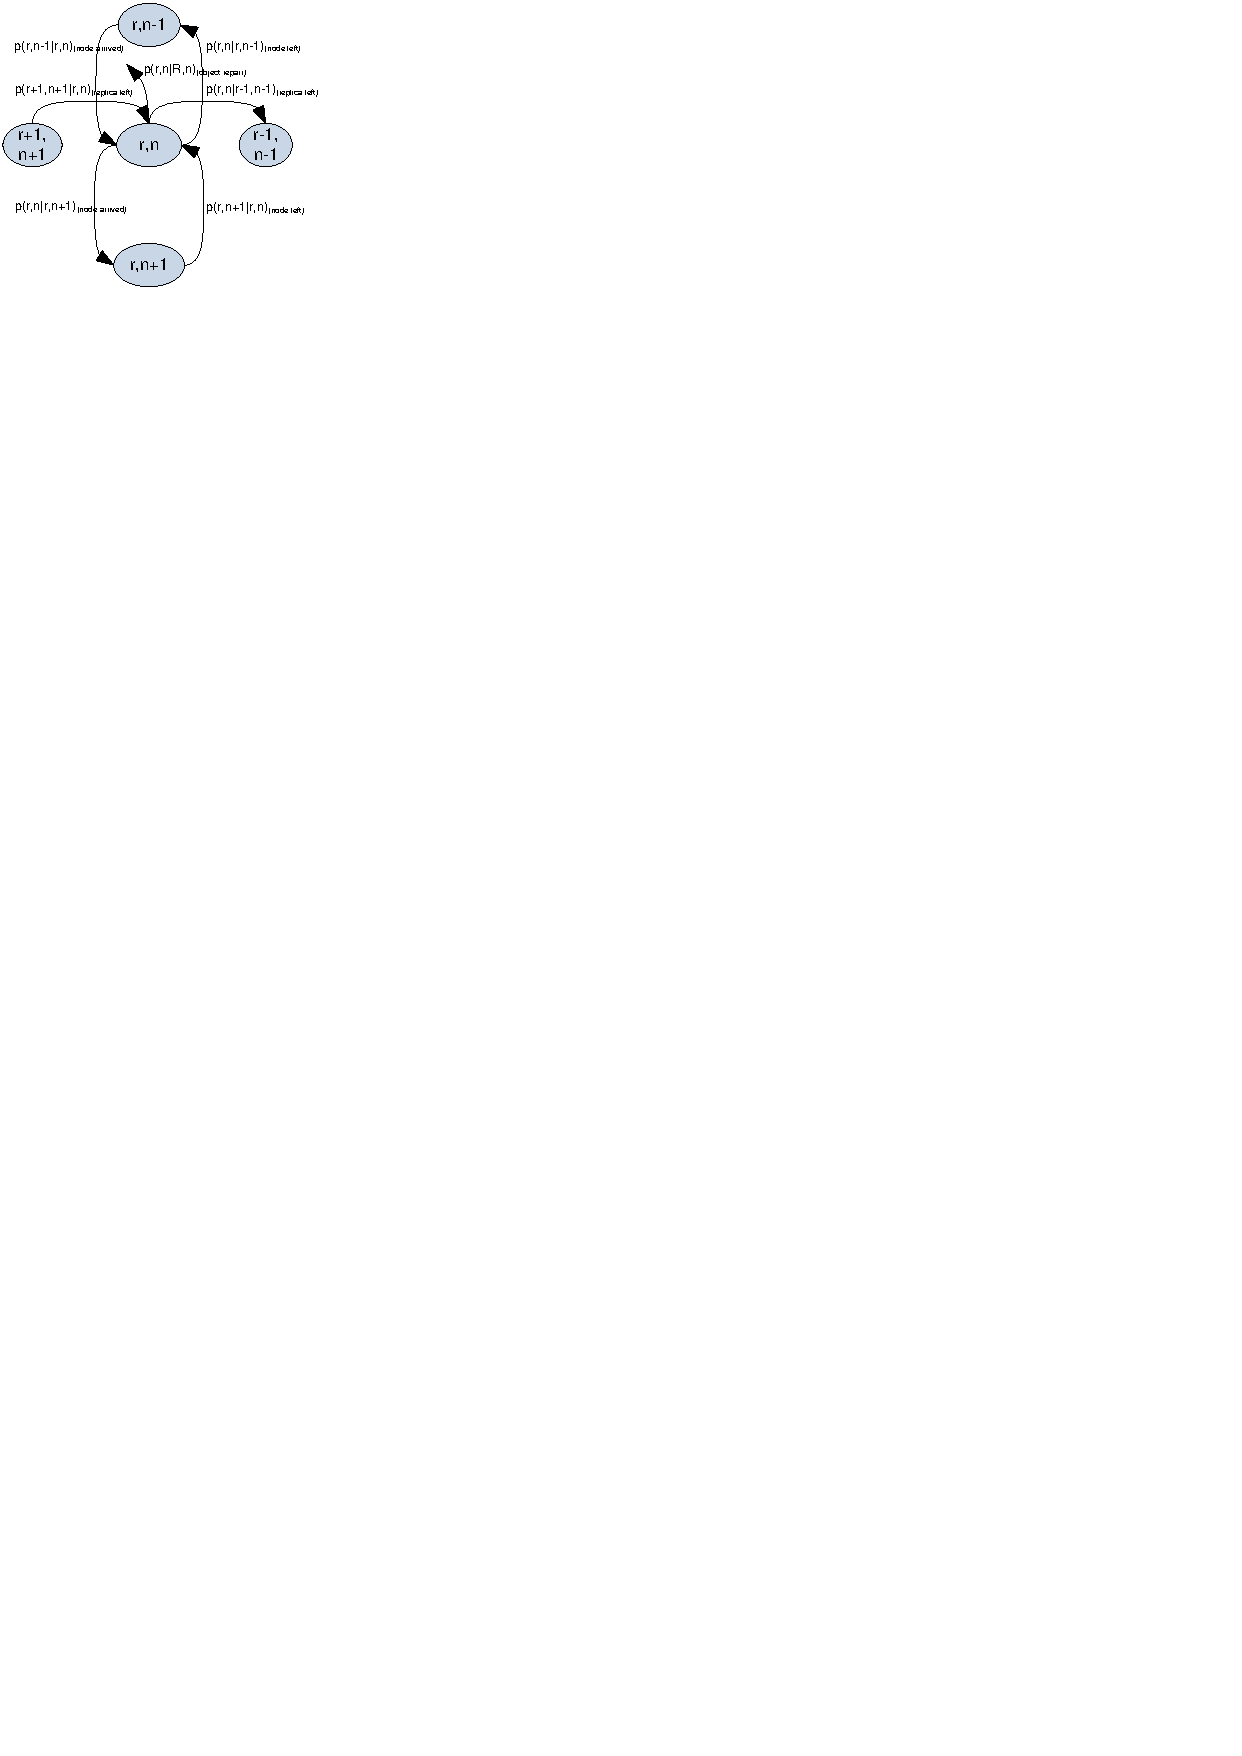
\includegraphics[clip=true, viewport=0.0cm 24.5cm 5.5cm 30cm, width=0.6\columnwidth]{Markov_example_syms}
 \caption{Markov chain modeling object replica number as well as network size, where $n-1\geqq R$ and $r > 1$}
 \label{fig_markov_example_syms}
\end{figure}

State transitions can be explained by the example in Figure \ref{fig_markov_example_syms}. The figure shows all state transitions relative to the centre state ($r,n$), which represents a state with $r$ replicas and $n$ nodes. For the purposes of explanation, only transitions to and from the centre state are shown. Starting at state ($r+1,n+1$), where $r+1$ replicas and $n+1$ nodes are present: If a node that contains a replica departs the network, the system moves to state ($r,n$): one fewer replica and one fewer node.

If a node that does not contain a replica now departs from the network, the system moves from state ($r,n$) to ($r,n-1$): no fewer replicas and one fewer node. A node can join the network, which will have the model move from ($r,n-1$) to ($r,n$) and another node joining the network will move the system into state ($r,n+1$).

The periodic repair mechanism, introduced in Section \ref{model_related_work} is also present. With sufficient nodes available for a full repair, the system moves from state ($r,n$) to ($R,n$). When the network size is smaller than the required number of replicas ($n<R$), the system moves to the state ($n,n$) instead, since there cannot be more replicas in the system than nodes.

\subsubsection{State transition rates}
\label{state_transition_rates}

For dual states, state transition rates are characterised by moving from state $i k$ to state $j l$, where $i$ is the number of replicas in the current state, $k$ the number of nodes in the current state, $j$ the number of replicas in the next state, and $l$ the number of nodes in the next state. Every state transition rate can then be expressed as a dual state transition equation.

Let $\theta$ be the departure rate of nodes under steady state. For a current state of $i$ replicas, the departure rate of nodes containing replicas from the network is $i\theta$. This transition can be expressed in terms of the dual state transition equation:
%
\begin{equation} \label{eq_rep_left}
    p(i k,j l)_{(\textrm{replica left})} = i\theta,\quad\textrm{for}\quad j = i - 1,\quad l = k - 1,
\end{equation}
%
where the next state contains one fewer replica and one fewer node than the current state.

The departure rate of nodes not containing replicas is the difference between the number of nodes currently in the network $k$ and the number of replicas currently in the network $i$. The departure rate is then $(k - i)\theta$ and the transition is given by
%
\begin{equation} \label{eq_node_left}
    p(i k,j l)_{(\textrm{node left})} = (k - i)\theta,\quad\textrm{for}\quad j = i,\quad l = k - 1,
\end{equation}
%
where the next state contains one fewer node, but the same number of replicas as the current state.

The Markov model assumes the presence of a finite sized network, with some maximum number of nodes $N$. The departure rate of nodes from the network is dependant on the number of nodes in the network. Similarly, if a maximum network size is assumed, the arrival rate of nodes in the network can be modelled as a function of nodes \emph{not} in the network. This creates a symmetry between the network departure and arrival rates, which creates a ``force'' in the Markov model that pushes the network to some average network size $\tilde{n}$, which is a ratio of $\theta$ to $\phi$. A stationary average network size is required to model a steady state network.

The arrival rate of nodes can thus be modelled as $(N - k)\phi$, the product of a single node arrival rate and the number of nodes not currently in the network, as given by
%
\begin{equation} \label{eq_node_arrived}
    p(i k,j l)_{(\textrm{node arrived})} = (N - k)\phi,\quad\textrm{for}\quad j = i,\quad l = k + 1,
\end{equation}
%
where the next state contains one more node, but the same number of replicas as the current state.

%Perhaps add some graphs here to show how node departure and arrival rate change with changes in network size. Show a graph or equation that will show the trend towards a single average. Perhaps use something like the rate difference to show force towards the centre.

$N$ should be chosen sufficiently large, compared to the average network size $\tilde{n}$, to ensure that the probability of the network model ever reaching $N$ is negligible. What constitutes a sufficiently large maximum network size will be evident from the results presented in Section \ref{results}. This requires that the ratios of $\theta$ to $\phi$ be chosen to produce a network with an average network size significantly smaller than $N$.

It is assumed that the repair mechanism repairs objects once every $T_{\textrm{repair}}$ time or at a rate of $\mu = 1/T_{\textrm{repair}}$, which gives
%
\begin{equation} \label{eq_repair}
    p(i k,j l)_{(\textrm{object repair})} = \mu,\quad\textrm{for}\quad j = \min(R, l),\quad l = k,\quad i \neq j.
\end{equation}
%
The number of replicas in the next state is either equal to the required number of replicas or the current number of nodes, whichever one is smallest, and the number of nodes remain the same as in the current state. When no replicas are missing, no repair occurs.

No transitions other than the ones described above can occur in the presented Markov model, therefore $p(i k,j l) = 0$ for all other state transitions.

\begin{figure}[htbp]
 \centering
 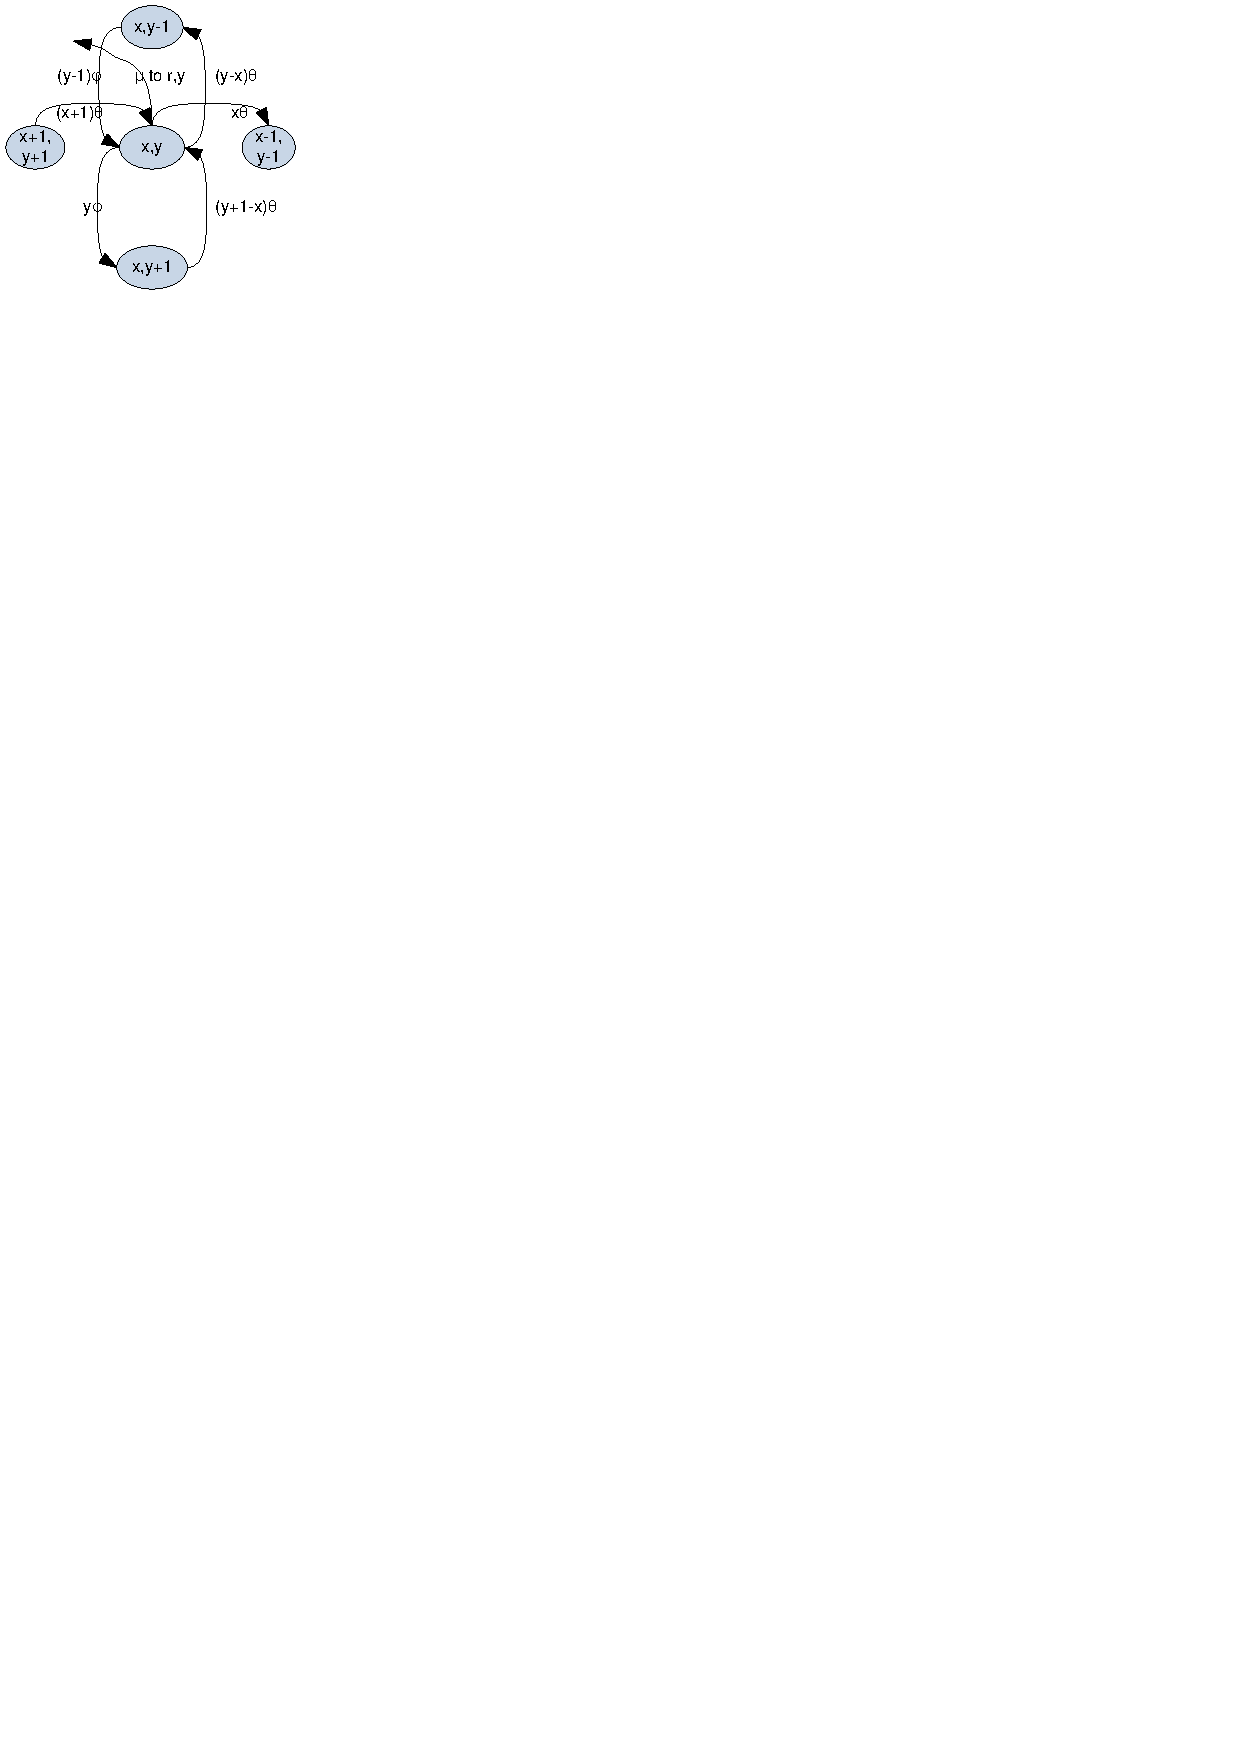
\includegraphics[clip=true, viewport=0.0cm 24.5cm 5.0cm 30cm, width=0.6\columnwidth]{Markov_example}
 \caption{Markov chain modeling object replica number as well as network size, where $n-1\geqq R$ and $r > 1$.}
 \label{fig_markov_example}
\end{figure}
%
Figure \ref{fig_markov_example} shows the example Markov chain shown earlier with the transition rates as described for the example. Apart from the example model developed, the initial states and absorbtion states have also been identified. The place bounds on the final Markov chain. An edge case has also been identified when there are too few nodes to perform a full repair. This limits the extent to which a repair can cause a state transition in the model.

\begin{figure}[htbp]
 \centering
 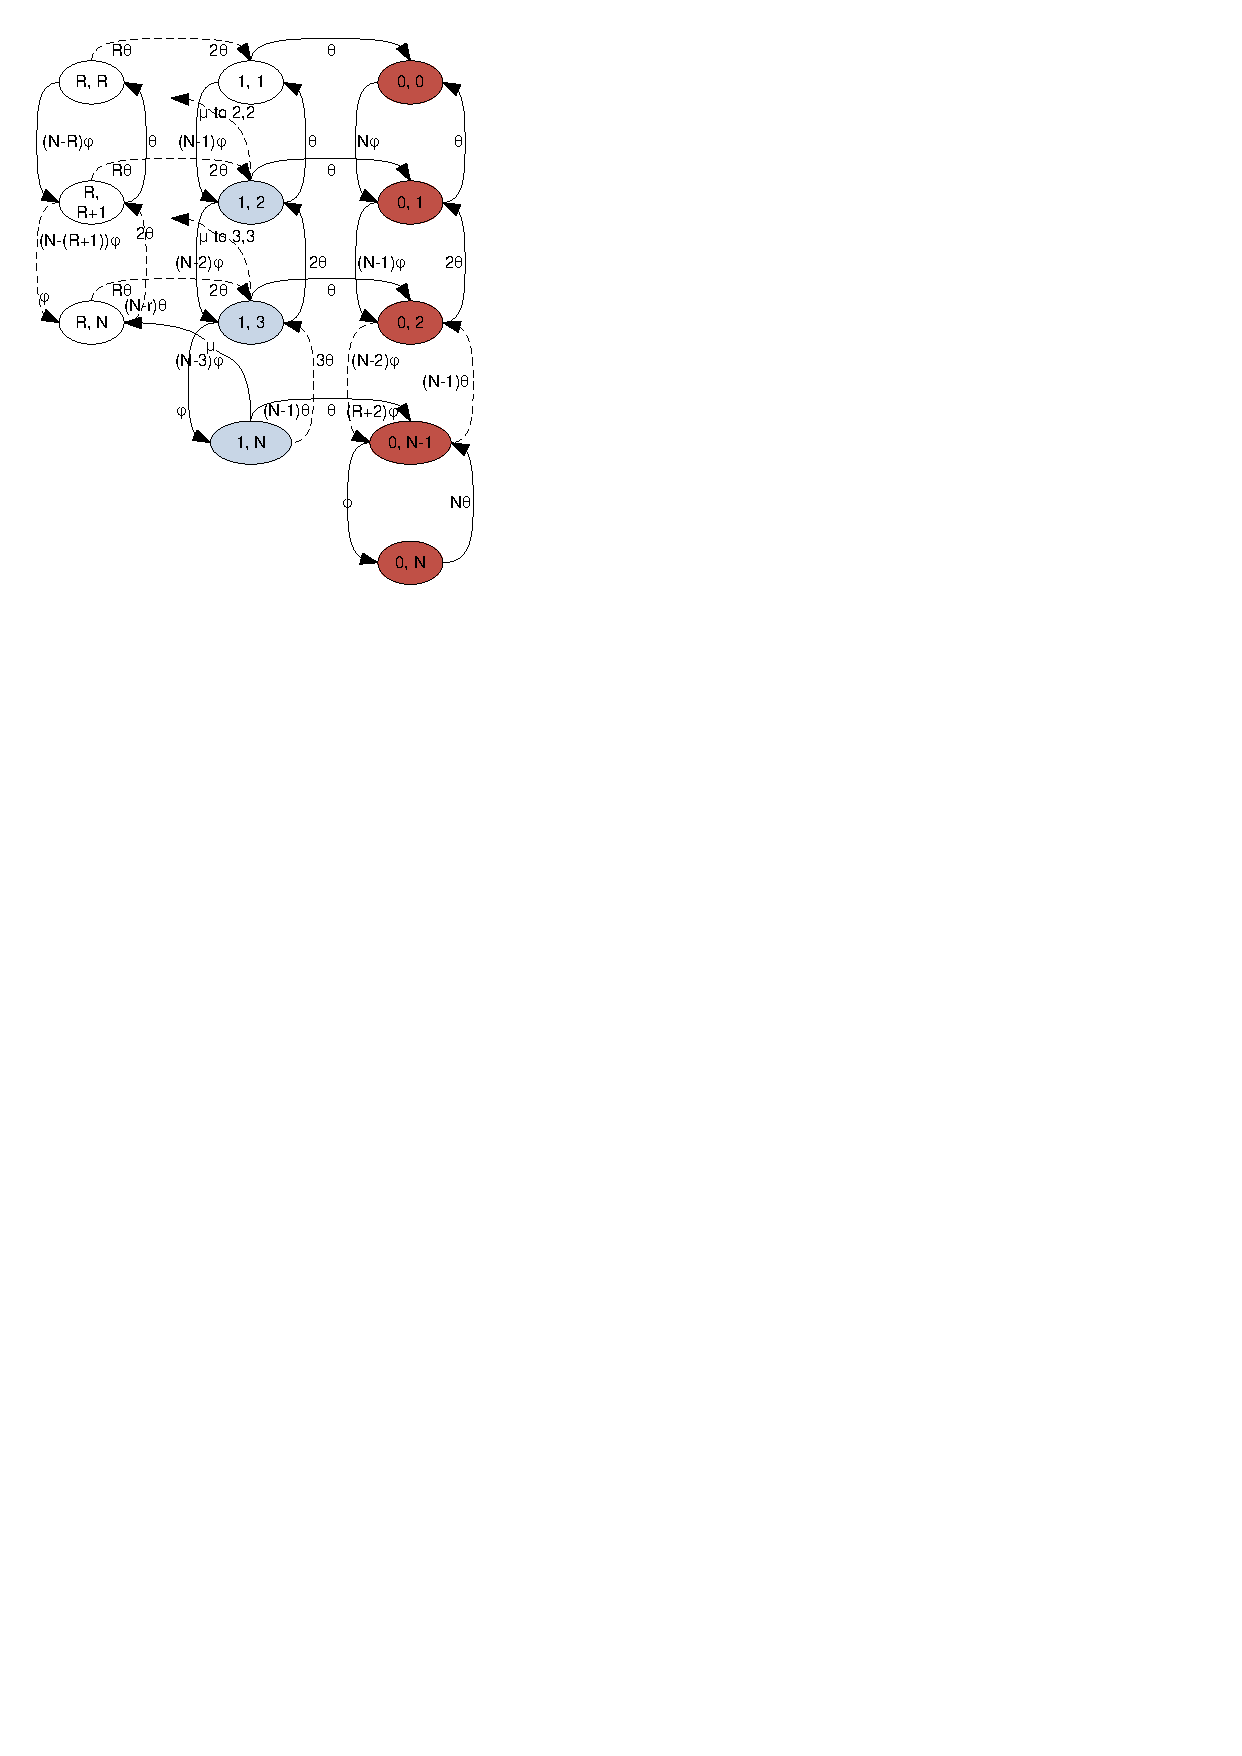
\includegraphics[clip=true, viewport=0.5cm 19.5cm 8.5cm 29.5cm, width=0.7\columnwidth]{Markov_chain_repair_compact}
 \caption{Markov chain modeling object replica number as well as network size and taking into account initial states, absorbtion states and the edge case of the network size limiting the replica number.}
 \label{fig_markov_chain}
\end{figure}
%
When these three aspects are taken into account, a Markov model of the form shown in Figure \ref{fig_markov_chain} is described. State transitions from one state to a consecutive state are shown by solid lines and transitions from one state to another state that contains intermediate state are shown by dashed lines. For dashed lines, to transition probabilities are shown: the transition probability from the source state and the transition probability to the destination state. The exception here is repair that has a fixed transition probability of $\mu$. For repair, the destination state is also given.

In Figure \ref{fig_markov_chain}, white states are initial states, red states are absorbtion states and blue states are neither initial nor absorbtion states. As explained earlier, initial state are state where the number of required replicas $r=R$ are inserted into the network if $n\geq R$, or where number of replicas equal to the number of nodes $r=n$ are inserted into the network if $n < R$. Absorbtion states are where no more object replicas exist in the network. There is, therefore, no way for objects to be repaired from this state.

It is evident that this model is a finite state model when a maximum number of nodes are assumed. In the horizontal, it is bounded by the required number of replicas $R$ and in the vertical it is bounded by the maximum number of nodes $N$. It can also be seen that this model does not have a rectangular shape, since there can never be more replicas than nodes ($r\leq n$).

\subsubsection{Node departure rate}
\label{node_departure_rate}

The node departure rate $\theta$ can be calculated from the lifetime distributions of the nodes in the network. As in the related work discussed in Section \ref{model_related_work}, all node lifetimes are assumed to be statistically independent and exponentially distributed. The exponential distribution is characterised by the single ``rate'' parameter $\lambda$.

The departure rate of nodes correspond to the failure rate (also called the hazard rate) of the node lifetime distribution \cite{rausand2004systemreliability}. An advantage of the exponential distribution is its ``memoryless'' property, which has a constant failure rate $h = \lambda$. For nodes with exponential lifetime distributions, the node departure rate is therefore $\theta = \lambda$.

As discussed in Section \ref{exp_vs_pareto}, the Pareto distribution is also used in reliability engineering to model node lifetimes and might be a better fit to online session times than the exponential distribution. The issue with using the Pareto distribution to model node lifetimes is its variable failure rate. This means that for a Pareto distribution, the average node departure rate under steady state is a function of the lifetimes of the nodes in the network $\theta = h(x)$.

In the work by Wu, Tian and Ng \cite{replication_article}, an approximation is made for Pareto failure rate, given by $\theta=(\alpha-2)/\beta$, where $\alpha$ and $\beta$ are two parameters of the Pareto distribution. \footnote{No derivation is provided for the approximation and the approximation could also not be found in the cited book.} During the calculation of expected object lifetimes, the expected lifetimes were found to be sensitive to small changes in the value of $\theta$, which renders the approximation unusable for practical predictions using Pareto lifetimes.

\subsubsection{Node arrival rate}

For the network to be in steady state, the average arrival rate of nodes must equal the average departure rate of nodes, which gives
%
\begin{equation}
    (N - \tilde{n})\phi = \tilde{n}\theta.\label{eq_phi_theta_ratio}
\end{equation}

Making $\phi$ the subject of Equation \eqref{eq_phi_theta_ratio} gives
%
\begin{equation}
    \phi = \frac{\tilde{n}\theta}{N - \tilde{n}},\label{eq_phi}
\end{equation}
%
which provides a value for $\phi$ that will produce a network with the desired average network size $\tilde{n}$, for a given $\theta$ and $N$.

\subsection{Number of states}

The Markov model presented, possesses a large number of states. To calculate the total number of states, two cases are identified. The first case is where the number of nodes in the network is greater or equal to the required number of replicas $k \geq R$. For every possible network size in this group, there are $R+1$ replica states. There are also $N - R + 1$ possible network sizes. From this it is evident that there are $(R+1)(N - R + 1)$ of these states in the Markov chain.

The second case is where the number of nodes in the network is fewer than the required number of replicas. For every possible network size in this case, the number of states are equal to the number of nodes in the network, going from $R$ to 1.

The total number of states is the sum of the two cases and is given by
%
\begin{align}
       S & = (R+1)(N - R + 1) + \sum_{x=1}^{R} x\label{eq_states_num_init}\\
         & = R(N - R + 1) + 0.5 (R + 1) R\notag\\
         & = 0.5 (R + 1) (2 N - R + 2), \quad\textrm{where}\quad N \geq R. \label{eq_states_num_ans}
\end{align}

For the size of network that Pithos was simulated for with 2500 nodes and 6 replicas per object, the resulting Markov chain contains 17486 states. The large number of states makes a closed form solution to the object lifetime problem intractable. Fortunately, numerical methods can be used to calculate object lifetimes for given numbers of replicas and maximum node sizes.

When calculating absorbtion times in the Markov chain, the number of transient states is also required. Transient states, as opposed to absorbtion states, are states out of which a transition can occur. In the model presented, all states containing zero replicas are absorbtion states. If the absorbtion states are removed, following the same process as with Equation \eqref{eq_states_num_ans}, but using $R$ instead of $R+1$ replica states, the number of transient states is given by
%
\begin{equation}
S_\textrm{transient} = 0.5 R (2 N - R + 1), \quad\textrm{where}\quad N \geq R. \label{eq_transient_states_num}
\end{equation}

Equation \eqref{eq_transient_states_num} can also be calculated by substituting $R-1$ into $R$ in Equation \eqref{eq_states_num_ans}.

\subsection{Calculating object lifetimes}

To calculate the expected object lifetimes, a transitional rates matrix is required for the Markov model presented. The number of rows and columns of the matrix are each equal to the total number of states in the Markov model. The transitional rates matrix contains the rate of movement from a source state $ik$ (represented by the row) to a destination state $jl$ (represented by the column). The transitional rates matrix contains the rates calculated in Section \ref{state_transition_rates} for all values of $p(ik, jl)$.

Since each element in the transitional rates matrix is a rate, the sum of all the elements in a single row of the rates matrix gives the rate of moving from that state to any other state. The inverse of this rate is the expected time $t_{ik}$ the Markov chain spends in state $ik$, given by
%
\begin{equation} \label{eq_markov_rates}
    t_{ik} = \left(\sum_{jl} p(ik, jl)\right)^{-1},
\end{equation}
%
which is the sum of all the columns of the transitional rates matrix for a specific row.

In an embedded Markov chain, the sum of all rows in the transitional rates matrix must equal one. This is achieved by normalising each row in the transitional rates matrix \textbf{P} to produce the normalised transitional rates matrix \textbf{\^{P}}, where each row in the matrix must satisfy
%
\begin{equation} \label{eq_markov_sum}
    \sum_{jl} \hat{p}(ik, jl) = 1.
\end{equation}

Using $t_{ik}$, \textbf{\^{P}} is given by
%
\begin{equation} \label{eq_markov_normalisation}
    \hat{p}(ik, jl) = p(ik, jl) t_{ik}.
\end{equation}

Object lifetime can be calculated by calculating the expected time to absorbtion of the embedded continuous time Markov chain. To do this, the normalised transitional rates matrix is partitioned into the form
%
\begin{equation} \label{matrix_partition}
    \textbf{\^{P}} = \left[\begin{array}{c|c}
                   \textbf{Q} & \textbf{R} \\
                   \hline
                   \textbf{0} & \textbf{I}
                 \end{array}\right].
\end{equation}
%
Every state transition can be considered a discrete event, which allows for the continuous time Markov chain to be embedded. This allows for theory from discrete time Markov chains to be used, with the exception that events are not equally spaced in time.

\textbf{\^{P}} is partitioned in such a way that all absorbing states are in the last rows and columns of \textbf{\^{P}}. Suppose there are $a$ absorbing states and $\tau$ transient states in the model. The matrix \textbf{Q} is then a $\tau\times\tau$ sub-matrix of \textbf{\^{P}} that contains all transient states. \textbf{I} is an $a \times a$ identity matrix, \textbf{0} is a $a\times\tau$ zero matrix and \textbf{R} (not to be confused with $R$) is a nonzero $\tau\times a$ matrix.

From \textbf{Q}, the fundamental matrix \textbf{N} may be calculated as \cite{grinstead1997introduction_probability}
%
\begin{equation} \label{eq_fundamental_mat}
    \textbf{N} = (\textbf{I} - \textbf{Q})^{-1}.
\end{equation}
%
Every element $n_{ik,jl}$ in the fundamental matrix \textbf{N} gives the expected number of times that the model is in the state $jl$, if it started in the transient state $ik$.

The expected time to absorbtion is then the product of the time spent in each state and the expected number of times a state will be entered, as given by
%
\begin{equation} \label{expected_lifetime}
    \textbf{E[L]} = \textbf{Nt},
\end{equation}
%
where \textbf{t} is the vector consisting of the times $t_{ik}$ for all $ik$.

\subsection{Example}

To illustrate how the developed equations can be used to calculate expected object lifetimes and to clarify the use of the equations to the reader, an example system is now shown, making use of the equations developed. To make the number of states manageable in the example, a network with a maximum size of $N=4$ nodes is used and $R=2$ replicas are required per object. Exponential node lifetimes are assumed with a mean node departure rate chosen as $\theta = \lambda = 0.5$. The mean network size is chosen as $\tilde{n} = 2$. The repair rate is chosen as $\mu = 0.01$.

It should be notes that because of the small number of nodes, the maximum network size $N$ is not significantly larger than the mean network size $\tilde{n}$, which reduces the accuracy of the results generated. The final results do still match intuitively between the number of replicas stored and object lifetime.

Equation \eqref{eq_phi} is used to calculate the node arrival rate using $N$, $\theta$ and $\tilde{n}$ as $\phi = \frac{2\times 0.5}{4-2} = 0.5$.

Equation \eqref{eq_repair} allows for the transitional rates matrix for object repair to be calculated as
%
\begin{equation}\label{eq_p_repair}
\textbf{P}_\textbf{repair} = \bbordermatrix{~
        & 2,4 & 1,4 & 0,4 & 2,3 & 1,3 & 0,3 & 2,2 & 1,2 & 0,2 & 1,1 & 0,1 & 0,0 \cr
    2,4 & 0   & 0   & 0   & 0   & 0   & 0   & 0   & 0   & 0   & 0   & 0   & 0 \cr
    1,4 & 0.01& 0   & 0   & 0   & 0   & 0   & 0   & 0   & 0   & 0   & 0   & 0 \cr
    0,4 & 0   & 0   & 0   & 0   & 0   & 0   & 0   & 0   & 0   & 0   & 0   & 0 \cr
    2,3 & 0   & 0   & 0   & 0   & 0   & 0   & 0   & 0   & 0   & 0   & 0   & 0 \cr
    1,3 & 0   & 0   & 0   & 0.01& 0   & 0   & 0   & 0   & 0   & 0   & 0   & 0 \cr
    0,3 & 0   & 0   & 0   & 0   & 0   & 0   & 0   & 0   & 0   & 0   & 0   & 0 \cr
    2,2 & 0   & 0   & 0   & 0   & 0   & 0   & 0   & 0   & 0   & 0   & 0   & 0 \cr
    1,2 & 0   & 0   & 0   & 0   & 0   & 0   & 0.01& 0   & 0   & 0   & 0   & 0 \cr
    0,2 & 0   & 0   & 0   & 0   & 0   & 0   & 0   & 0   & 0   & 0   & 0   & 0 \cr
    1,1 & 0   & 0   & 0   & 0   & 0   & 0   & 0   & 0   & 0   & 0   & 0   & 0 \cr
    0,1 & 0   & 0   & 0   & 0   & 0   & 0   & 0   & 0   & 0   & 0   & 0   & 0 \cr
    0,0 & 0   & 0   & 0   & 0   & 0   & 0   & 0   & 0   & 0   & 0   & 0   & 0 \cr
},
\end{equation}
%
where the matrix is bordered by the dual state that each row and column represents. A row of the matrix gives the source state a column gives the destination state. In the matrix in Equation \eqref{eq_p_repair}, it can be seen that repair occurs at a rate $\mu=0.01$ for a state with fewer than 2 replicas, moving to a state with the maximum allowed replicas, as described earlier.

Equation \eqref{eq_node_arrived} allows for the transitional rates matrix for node arrival to be calculated as
%
\begin{equation}
\textbf{P}_\textbf{node arrived} = \bbordermatrix{~
        & 2,4 & 1,4 & 0,4 & 2,3 & 1,3 & 0,3 & 2,2 & 1,2 & 0,2 & 1,1 & 0,1 & 0,0 \cr
    2,4 & 0   & 0   & 0   & 0   & 0   & 0   & 0   & 0   & 0   & 0   & 0   & 0 \cr
    1,4 & 0   & 0   & 0   & 0   & 0   & 0   & 0   & 0   & 0   & 0   & 0   & 0 \cr
    0,4 & 0   & 0   & 0   & 0   & 0   & 0   & 0   & 0   & 0   & 0   & 0   & 0 \cr
    2,3 & 0.5 & 0   & 0   & 0   & 0   & 0   & 0   & 0   & 0   & 0   & 0   & 0 \cr
    1,3 & 0   & 0.5 & 0   & 0   & 0   & 0   & 0   & 0   & 0   & 0   & 0   & 0 \cr
    0,3 & 0   & 0   & 0.5 & 0   & 0   & 0   & 0   & 0   & 0   & 0   & 0   & 0 \cr
    2,2 & 0   & 0   & 0   & 1   & 0   & 0   & 0   & 0   & 0   & 0   & 0   & 0 \cr
    1,2 & 0   & 0   & 0   & 0   & 1   & 0   & 0   & 0   & 0   & 0   & 0   & 0 \cr
    0,2 & 0   & 0   & 0   & 0   & 0   & 1   & 0   & 0   & 0   & 0   & 0   & 0 \cr
    1,1 & 0   & 0   & 0   & 0   & 0   & 0   & 0   & 1.5 & 0   & 0   & 0   & 0 \cr
    0,1 & 0   & 0   & 0   & 0   & 0   & 0   & 0   & 0   & 1.5 & 0   & 0   & 0 \cr
    0,0 & 0   & 0   & 0   & 0   & 0   & 0   & 0   & 0   & 0   & 0   & 2   & 0 \cr
}.
\end{equation}
%
A state transition occurs, moving to a state with one more node from any state that does not already possess the maximum number of nodes. For example, in the first column a state transition occurs from (2,3) to (2,4) at a rate of $(N-k)\phi = (4-3)\times 0.5 = 0.5$.

Equation \eqref{eq_rep_left} allows for the transitional rates matrix for replica departure to be calculated as
%
\begin{equation}
\textbf{P}_\textbf{replica left} = \bbordermatrix{~
        & 2,4 & 1,4 & 0,4 & 2,3 & 1,3 & 0,3 & 2,2 & 1,2 & 0,2 & 1,1 & 0,1 & 0,0 \cr
    2,4 & 0   & 0   & 0   & 0   & 1   & 0   & 0   & 0   & 0   & 0   & 0   & 0  \cr
    1,4 & 0   & 0   & 0   & 0   & 0   & 0.5 & 0   & 0   & 0   & 0   & 0   & 0  \cr
    0,4 & 0   & 0   & 0   & 0   & 0   & 0   & 0   & 0   & 0   & 0   & 0   & 0  \cr
    2,3 & 0   & 0   & 0   & 0   & 0   & 0   & 0   & 1   & 0   & 0   & 0   & 0  \cr
    1,3 & 0   & 0   & 0   & 0   & 0   & 0   & 0   & 0   & 0.5 & 0   & 0   & 0  \cr
    0,3 & 0   & 0   & 0   & 0   & 0   & 0   & 0   & 0   & 0   & 0   & 0   & 0  \cr
    2,2 & 0   & 0   & 0   & 0   & 0   & 0   & 0   & 0   & 0   & 1   & 0   & 0  \cr
    1,2 & 0   & 0   & 0   & 0   & 0   & 0   & 0   & 0   & 0   & 0   & 0.5 & 0  \cr
    0,2 & 0   & 0   & 0   & 0   & 0   & 0   & 0   & 0   & 0   & 0   & 0   & 0  \cr
    1,1 & 0   & 0   & 0   & 0   & 0   & 0   & 0   & 0   & 0   & 0   & 0   & 0.5\cr
    0,1 & 0   & 0   & 0   & 0   & 0   & 0   & 0   & 0   & 0   & 0   & 0   & 0  \cr
    0,0 & 0   & 0   & 0   & 0   & 0   & 0   & 0   & 0   & 0   & 0   & 0   & 0  \cr
}.
\end{equation}
%
A state transition occurs when moving from a state with more than one replicas to another state with one fewer replicas and one fewer nodes. An example transition occurs when moving from state (2,3) to state (1,2) at a rate of $i\theta = 2\times 0.5 = 1$.

Equation \eqref{eq_node_left} allows for the transitional rates matrix for node departure to be calculated as
%
\begin{equation}
\textbf{P}_\textbf{node left} = \bbordermatrix{~
        & 2,4 & 1,4 & 0,4 & 2,3 & 1,3 & 0,3 & 2,2 & 1,2 & 0,2 & 1,1 & 0,1 & 0,0 \cr
    2,4 & 0   & 0   & 0   & 1   & 0   & 0   & 0   & 0   & 0   & 0   & 0   & 0  \cr
    1,4 & 0   & 0   & 0   & 0   & 1.5 & 0   & 0   & 0   & 0   & 0   & 0   & 0  \cr
    0,4 & 0   & 0   & 0   & 0   & 0   & 2   & 0   & 0   & 0   & 0   & 0   & 0  \cr
    2,3 & 0   & 0   & 0   & 0   & 0   & 0   & 0.5 & 0   & 0   & 0   & 0   & 0  \cr
    1,3 & 0   & 0   & 0   & 0   & 0   & 0   & 0   & 1   & 0   & 0   & 0   & 0  \cr
    0,3 & 0   & 0   & 0   & 0   & 0   & 0   & 0   & 0   & 1.5 & 0   & 0   & 0  \cr
    2,2 & 0   & 0   & 0   & 0   & 0   & 0   & 0   & 0   & 0   & 0   & 0   & 0  \cr
    1,2 & 0   & 0   & 0   & 0   & 0   & 0   & 0   & 0   & 0   & 0.5 & 0   & 0  \cr
    0,2 & 0   & 0   & 0   & 0   & 0   & 0   & 0   & 0   & 0   & 0   & 1   & 0  \cr
    1,1 & 0   & 0   & 0   & 0   & 0   & 0   & 0   & 0   & 0   & 0   & 0   & 0  \cr
    0,1 & 0   & 0   & 0   & 0   & 0   & 0   & 0   & 0   & 0   & 0   & 0   & 0.5\cr
    0,0 & 0   & 0   & 0   & 0   & 0   & 0   & 0   & 0   & 0   & 0   & 0   & 0  \cr
}.
\end{equation}
%
A state transition occurs when from a state with more than zero nodes to a state with one more node and no more replicas. An example transition occurs when moving from state (0,4) to (0,3) at a rate of $(k-i)\theta = (4-0)\theta = 2$.

The final transitional rates matrix may be obtained by the sum of the previous transitional rates matrices $\textbf{P} = \textbf{P}_\textbf{repair} + \textbf{P}_\textbf{node arrived} + \textbf{P}_\textbf{replica left} + \textbf{P}_\textbf{node left}$, which gives
%
\begin{equation}
\textbf{P} = \bbordermatrix{~
        & 2,4 & 1,4 & 0,4 & 2,3 & 1,3 & 0,3 & 2,2 & 1,2 & 0,2 & 1,1 & 0,1 & 0,0 \cr
    2,4 & 0   & 0   & 0   & 1   & 1   & 0   & 0   & 0   & 0   & 0   & 0   & 0 \cr
    1,4 & 0.01& 0   & 0   & 0   & 1.5 & 0.5 & 0   & 0   & 0   & 0   & 0   & 0 \cr
    0,4 & 0   & 0   & 0   & 0   & 0   & 2   & 0   & 0   & 0   & 0   & 0   & 0 \cr
    2,3 & 0.5 & 0   & 0   & 0   & 0   & 0   & 0.5 & 1   & 0   & 0   & 0   & 0 \cr
    1,3 & 0   & 0.5 & 0   & 0.01& 0   & 0   & 0   & 1   & 0.5 & 0   & 0   & 0 \cr
    0,3 & 0   & 0   & 0.5 & 0   & 0   & 0   & 0   & 0   & 1.5 & 0   & 0   & 0 \cr
    2,2 & 0   & 0   & 0   & 1   & 0   & 0   & 0   & 0   & 0   & 1   & 0   & 0 \cr
    1,2 & 0   & 0   & 0   & 0   & 1   & 0   & 0.01& 0   & 0   & 0.5 & 0.5 & 0 \cr
    0,2 & 0   & 0   & 0   & 0   & 0   & 1   & 0   & 0   & 0   & 0   & 1   & 0 \cr
    1,1 & 0   & 0   & 0   & 0   & 0   & 0   & 0   & 1.5 & 0   & 0   & 0   & 0.5\cr
    0,1 & 0   & 0   & 0   & 0   & 0   & 0   & 0   & 0   & 1.5 & 0   & 0   & 0.5\cr
    0,0 & 0   & 0   & 0   & 0   & 0   & 0   & 0   & 0   & 0   & 0   & 2   & 0 \cr
}.
\end{equation}

%\begin{equation}
%\textbf{\^{P}} = \bbordermatrix{~
%        & 2,4 & 1,4 & 0,4 & 2,3 & 1,3 & 0,3 & 2,2 & 1,2 & 0,2 & 1,1 & 0,1 & 0,0 \cr
%    2,4 & 0   & 0   & 0   & 0.5 & 0.5 & 0   & 0   & 0   & 0   & 0   & 0   & 0 \cr
%    1,4 &0.005& 0   & 0   & 0   &0.7463&0.2488& 0   & 0   & 0   & 0   & 0   & 0 \cr
%    0,4 & 0   & 0   & 0   & 0   & 0   & 1   & 0   & 0   & 0   & 0   & 0   & 0 \cr
%    2,3 & 0.25& 0   & 0   & 0   & 0   & 0   & 0.25& 0.5 & 0   & 0   & 0   & 0 \cr
%    1,3 & 0   &0.2488& 0   &0.005& 0   & 0   & 0   &0.4976&0.2488& 0   & 0   & 0 \cr
%    0,3 & 0   & 0   & 0.25& 0   & 0   & 0   & 0   & 0   & 0.75& 0   & 0   & 0 \cr
%    2,2 & 0   & 0   & 0   & 0.5 & 0   & 0   & 0   & 0   & 0   & 0.5   & 0   & 0 \cr
%    1,2 & 0   & 0   & 0   & 0   &0.4975& 0   &0.005& 0   & 0   &0.2488&0.2488& 0 \cr
%    0,2 & 0   & 0   & 0   & 0   & 0   & 0.5   & 0   & 0   & 0   & 0   & 0.5   & 0 \cr
%    1,1 & 0   & 0   & 0   & 0   & 0   & 0   & 0   &0.75& 0   & 0   & 0   & 0.25\cr
%    0,1 & 0   & 0   & 0   & 0   & 0   & 0   & 0   & 0   & 0.75 & 0   & 0   & 0.25\cr
%    0,0 & 0   & 0   & 0   & 0   & 0   & 0   & 0   & 0   & 0   & 0   & 1   & 0 \cr
%}
%\end{equation}

The rates vector can then be calculated from the transitional rates matrix making use of Equation \eqref{eq_markov_rates}, which gives
%
\begin{equation}\label{rates_vector_example}
\textbf{t} = \bbordermatrix{~
    &\cr
    2,4 &0.5000\cr
    1,4 &0.4975\cr
    2,3 &0.5000\cr
    1,3 &0.4975\cr
    2,2 &0.5000\cr
    1,2 &0.4975\cr
    1,1 &0.5000\cr
}.
\end{equation}

The transitional rates matrix is then normalised using Equation \eqref{eq_markov_normalisation} and the rates vector $\textbf{t}$ produced by Equation \eqref{rates_vector_example}. The normalised transitional rates matrix $\textbf{\^{P}}$ is than partitioned as described in Equation \eqref{matrix_partition} and the transient normalised transitional rates matrix is created, given by
%
\begin{equation}
\textbf{Q} = \bbordermatrix{~
        & 2,4 & 1,4  & 2,3 & 1,3  & 2,2  & 1,2  & 1,1   \cr
    2,4 & 0   & 0    & 0.5 & 0.5  & 0    & 0    & 0     \cr
    1,4 &0.005& 0    & 0   &0.7463& 0    & 0    & 0     \cr
    2,3 & 0.25& 0    & 0   & 0    & 0.25 & 0.5  & 0     \cr
    1,3 & 0   &0.2488&0.005& 0    & 0    &0.4976& 0     \cr
    2,2 & 0   & 0    & 0.5 & 0    & 0    & 0    & 0.5   \cr
    1,2 & 0   & 0    & 0   &0.4975& 0.005& 0    & 0.2488\cr
    1,1 & 0   & 0    & 0   & 0    & 0    &0.75  & 0     \cr
}.
\end{equation}
%
The transient normalised transitional rates matrix $\textbf{Q}$ can be calculated by simply removing all rows and columns where there are zero replicas from the normalised transitional rates matrix $\textbf{\^{P}}$. Take note that most rows in $\textbf{Q}$ sum to one, but that some do not. These are where an absorbtion state was removed. When taking the absorbtion state into account, all rows sum to one.

The fundamental matrix can then by calculated by Equation \ref{eq_fundamental_mat}, which gives
%
\begin{equation}\label{fundamental_matrix_example}
\textbf{N} = \bbordermatrix{~
        & 2,4   & 1,4     & 2,3     & 1,3     & 2,2     & 1,2     & 1,1   \cr
    2,4 &1.1730 &  0.4080 &  0.6839 &  1.6401 &  0.1785 &  1.5058 &  0.4638\cr
    1,4 &0.0112 &  1.3703 &  0.0175 &  1.4886 &  0.0090 &  0.9253 &  0.2347\cr
    2,3 &0.3388 &  0.3225 &  1.3489 &  1.2965 &  0.3461 &  1.7817 &  0.6162\cr
    1,3 &0.0072 &  0.4935 &  0.0189 &  1.9837 &  0.0108 &  1.2299 &  0.3114\cr
    2,2 &0.1715 &  0.2751 &  0.6803 &  1.1058 &  1.1782 &  1.6377 &  0.9965\cr
    1,2 &0.0054 &  0.3035 &  0.0157 &  1.2201 &  0.0138 &  1.9916 &  0.5023\cr
    1,1 &0.0041 &  0.2276 &  0.0118 &  0.9150 &  0.0104 &  1.4937 &  1.3768\cr
}.
\end{equation}

The expected node lifetimes, for every initial state, can then be calculated using Equation \eqref{expected_lifetime} and the results from Equations \eqref{rates_vector_example} and \eqref{fundamental_matrix_example}, which gives
%
\begin{equation}\label{expected_lifetimes_example}
\textbf{E[L]} = \bbordermatrix{~
    &\cr
    2,4 &3.0177\cr
    1,4 &2.0188\cr
    2,3 &3.0169\cr
    1,3 &2.0184\cr
    2,2 &3.0150\cr
    1,2 &2.0175\cr
    1,1 &2.0131\cr
}.
\end{equation}

\begin{table}[htbp]
\centering
\begin{tabular}{|c|c|c|c|c|}
\hline
            & \textbf{2 replicas} & \textbf{1 replica} \\
\hline
 \textbf{4 nodes} & 3             & 2          \\
 \textbf{3 nodes} & 3             & 2          \\
 \textbf{2 nodes} & 3             & 2          \\
 \textbf{1 node} &                & 2          \\
\hline
\end{tabular}
\caption{Table showing expected object lifetimes for the number of nodes and replicas calculated in the example.}
\label{tab_lifetimes_example}
\end{table}
%
Table \ref{tab_lifetimes_example} shows the results from Equation \eqref{expected_lifetimes_example}, rounded and reorganised by number of nodes and number of replicas. The results generated shows that an object for which 2 replicas were stored lives longer than an object for which a single replica was stored, which is as expected.

\section{Model results}
\label{results}

The simulation model will now be explored for larger numbers of objects and replicas to get an understanding of how the various network parameters influence object lifetime. For all results presented in this section, the following parameter values are used: a maximum network size of $N=120$, a required number of replicas of $R = 10$ and exponential node lifetime distributions with $\lambda = \theta = 1/1800$, which gives expected \emph{node} lifetimes of $1/\lambda = 1800$ seconds.

It should be noted that the geometry of the practical network is not important for the model developed in this chapter. All that should be ensured is that objects are replicated and repaired as assumed in the model. The purpose of this chapter is, however, to investigate object lifetimes in Pithos groups. This is why a focus was placed on finite sized networks, since Pithos groups are often size limited. Which means that the size of a Pithos groups is comparable to the number of required object replicas. This is why a model assuming an infinite sized network is not applicable to Pithos.

During an investigation of the model, it was found that for the maximum network size $N$ to be sufficiently large, it does not have to be many orders of magnitude higher than the average network size presented. The choice of $N=120$ is the smallest number of nodes that no longer have an influence on the maximum average group size of $\tilde{n}=50$ being investigated in this section. It is preferable to choose the smallest possible maximum network size to minimise the state explosion of the Markov model and thereby allowing modern desktop computers to calculate the expected node lifetimes successfully.

\begin{figure}[htbp]
 \centering
 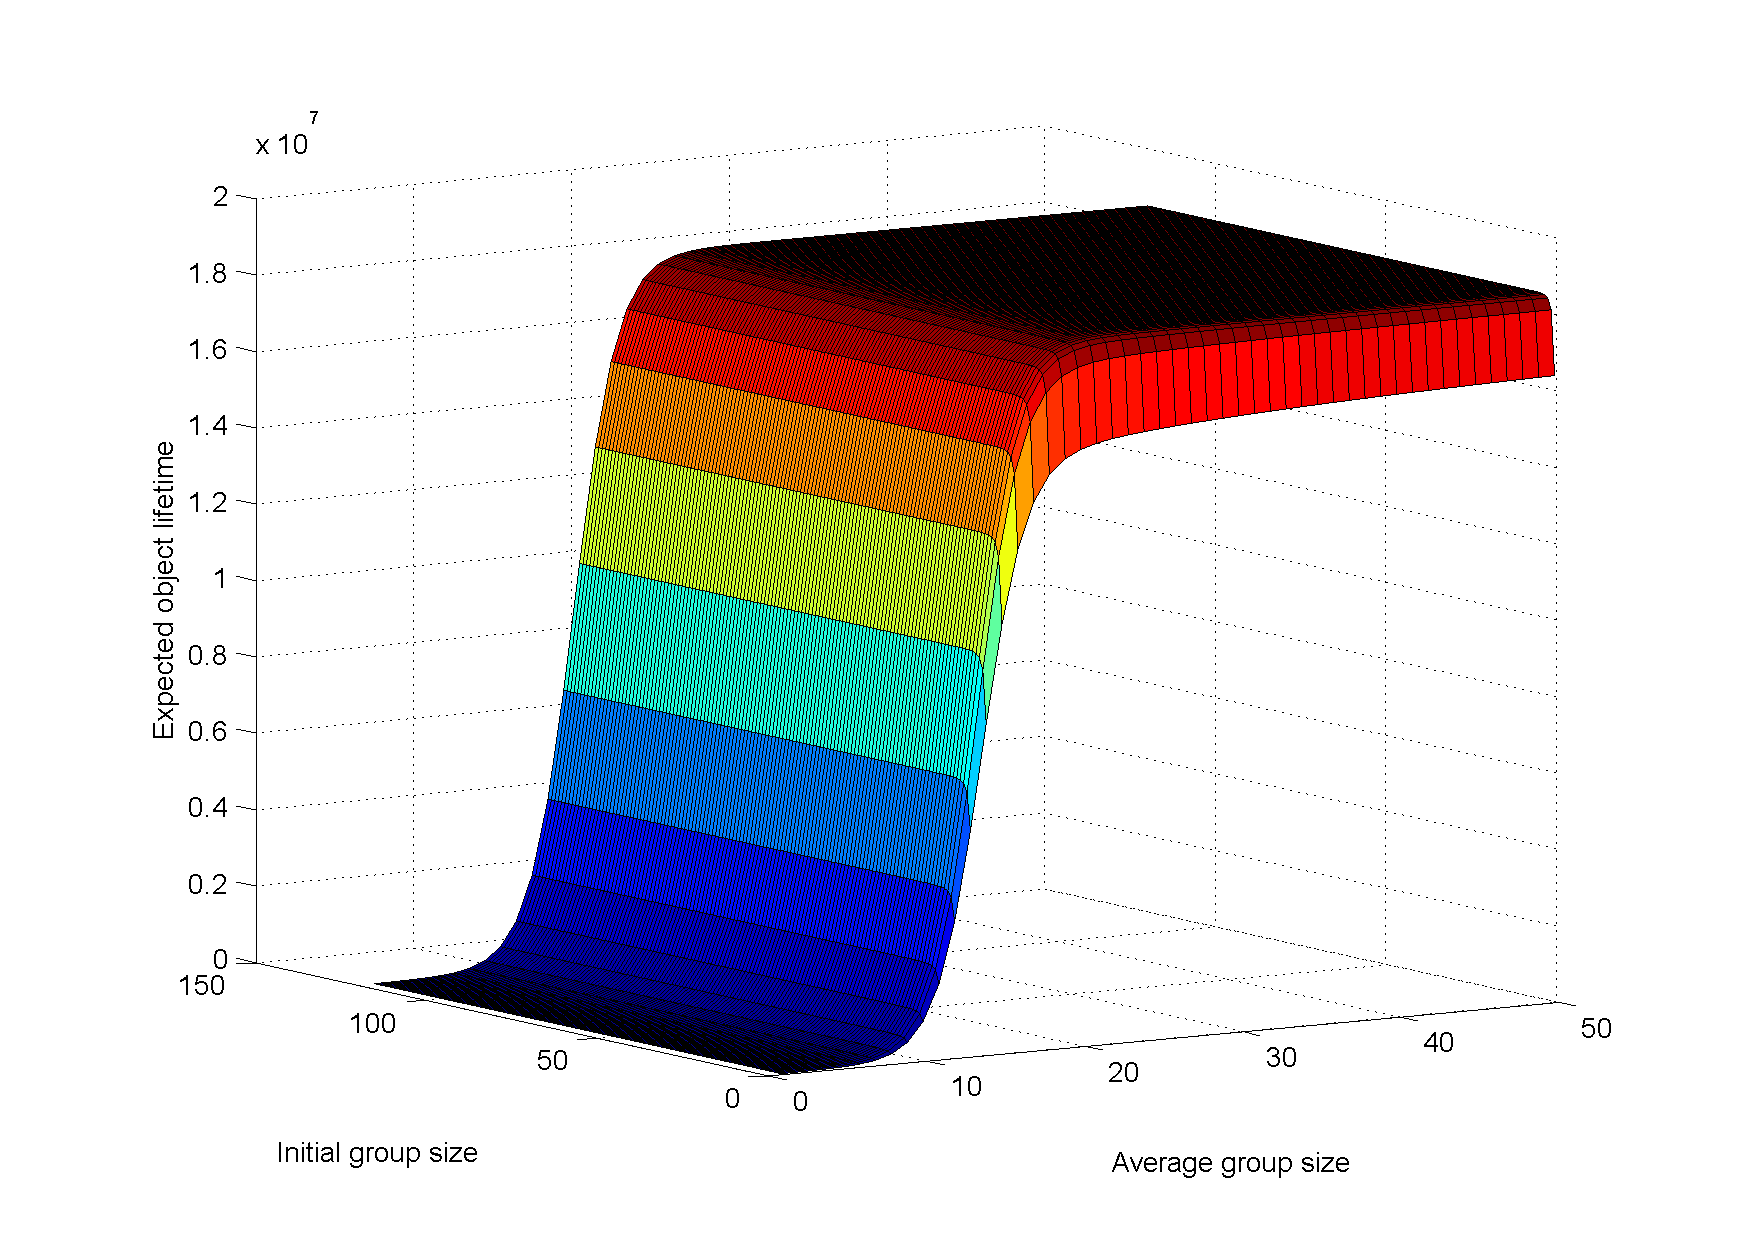
\includegraphics[clip=true, viewport=1.5cm 3.5cm 28.0cm 16.5cm, width=\columnwidth]{lifetime_av_init_groupsize}
 \caption{Surface plots of expected object lifetimes as functions of initial and average network sizes for $\mu = 1/180$ (above) and $\mu = 0$ (below).}
 \label{fig_lifetime_average_vs_initial}
\end{figure}
%
Figure \ref{fig_lifetime_average_vs_initial} shows surface plots of expected object lifetimes against initial and average network sizes for a repair rate of $\mu = 1/180$ (or $T_{\textrm{repair}}$ $10\%$ of the expected node lifetime) and no repair rate. It is evident that object lifetimes decrease greatly for average network sizes smaller than 20 nodes for the case with repair, but that average network size has no effect when repair is not used. The model presented in this chapter shows a significant decrease in expected lifetime every time the average network size is comparable to the required number of replicas, for the case with repair. The figure also shows that expected object lifetimes decrease when the initial network size is smaller than the required number of replicas. From the figure it can also be seen that initial network size has a more pronounced effect on the expected object lifetime, when no repair is used than when repair is used.

\begin{figure}[htbp]
 \centering
 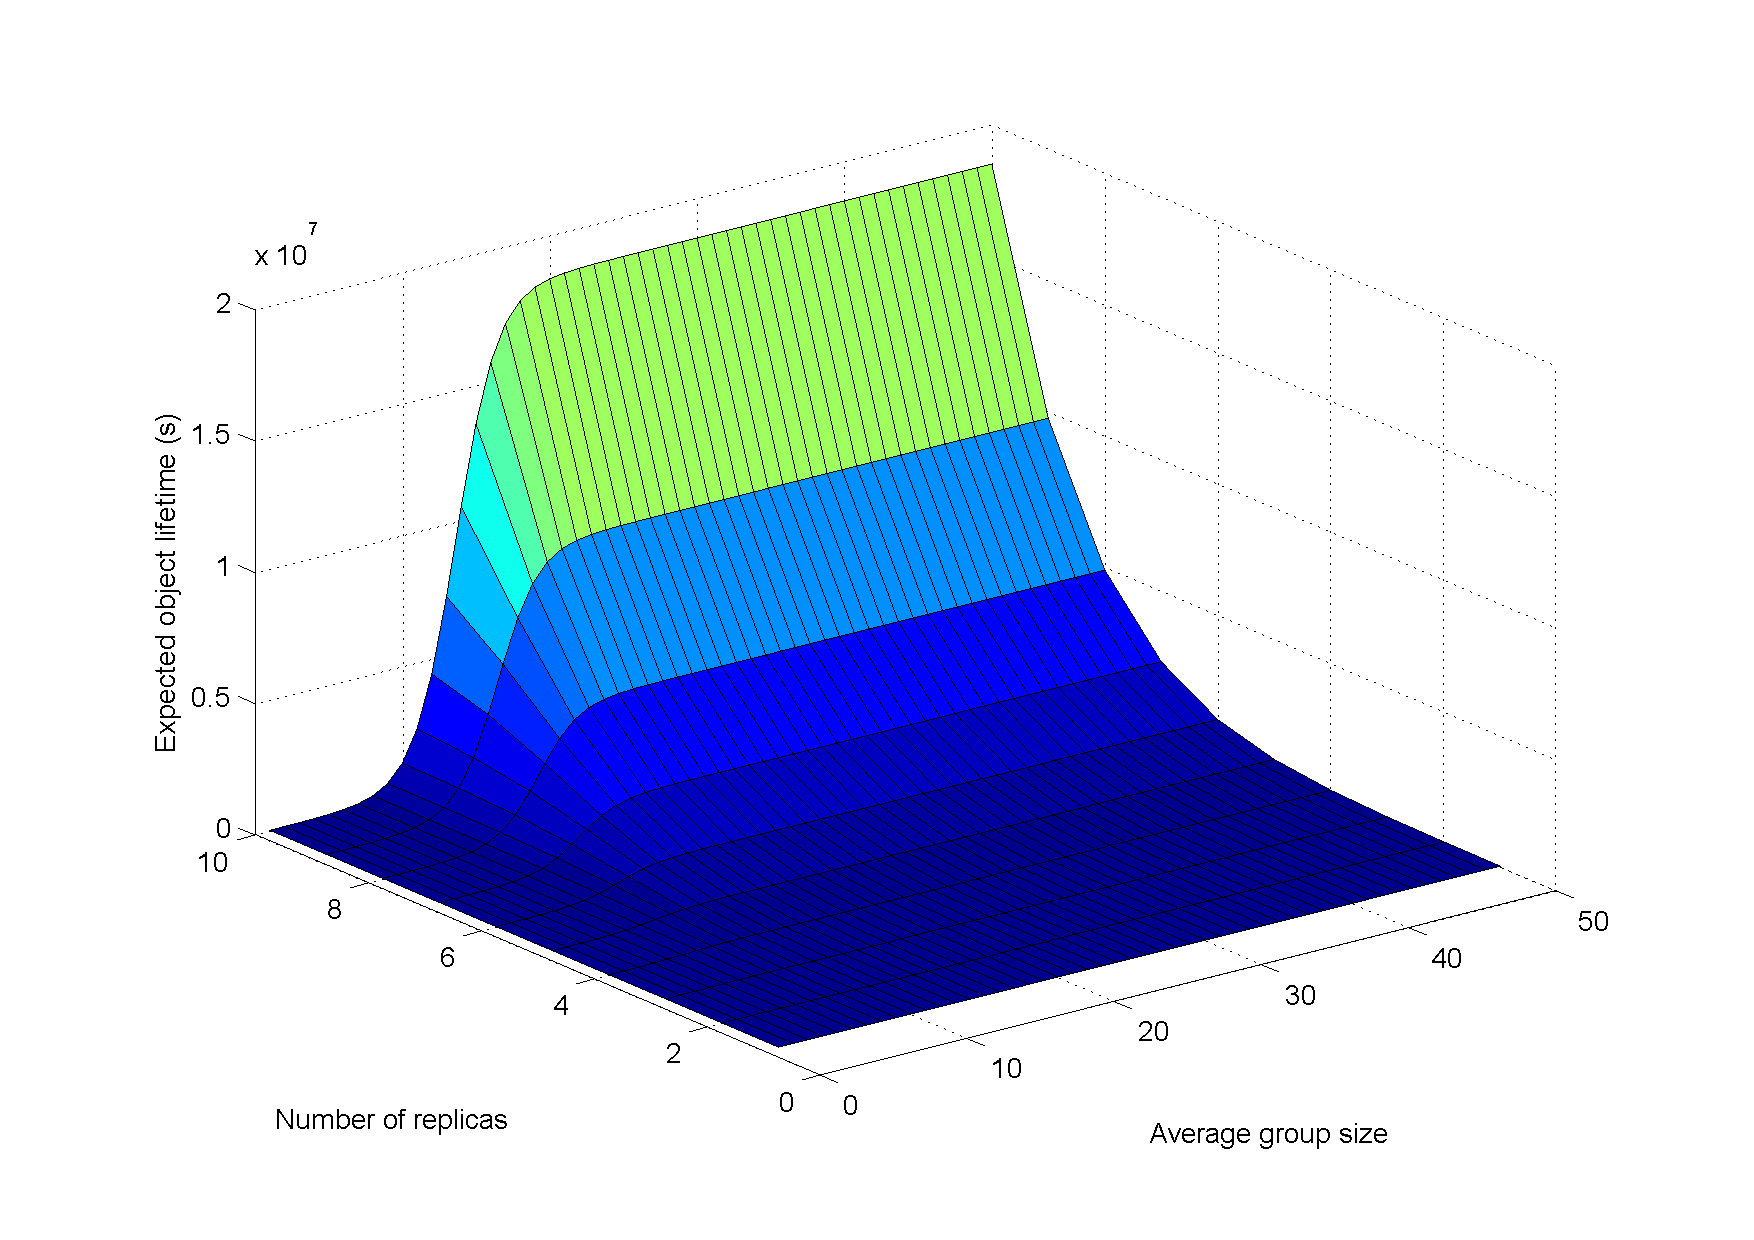
\includegraphics[clip=true, viewport=2.5cm 1.0cm 27.5cm 19.15cm, width=0.8\columnwidth]{lifetime_replicas_av_groupsize}
 \caption{Surface plot of expected object lifetimes as functions of average network size and required number of replicas $R$ for $mu = 1/180$.}
 \label{fig_lifetime_average_vs_replicas}
\end{figure}
%
Figure \ref{fig_lifetime_average_vs_replicas} depicts the expected object lifetime as functions of average network size and required number of replicas $R$ for a repair rate of $\mu = 1/180$. To generate this figure, $R$ is swept from 1 to 10 to illustrate the effect that an increase in the number of replicas has on the expected node lifetime. The figure shows that an increase in $R$ leads to an exponential increase in the expected object lifetime, but that this gain is limited when the average network size is small, compared to the required number of replicas.

\begin{figure}[htbp]
 \centering
 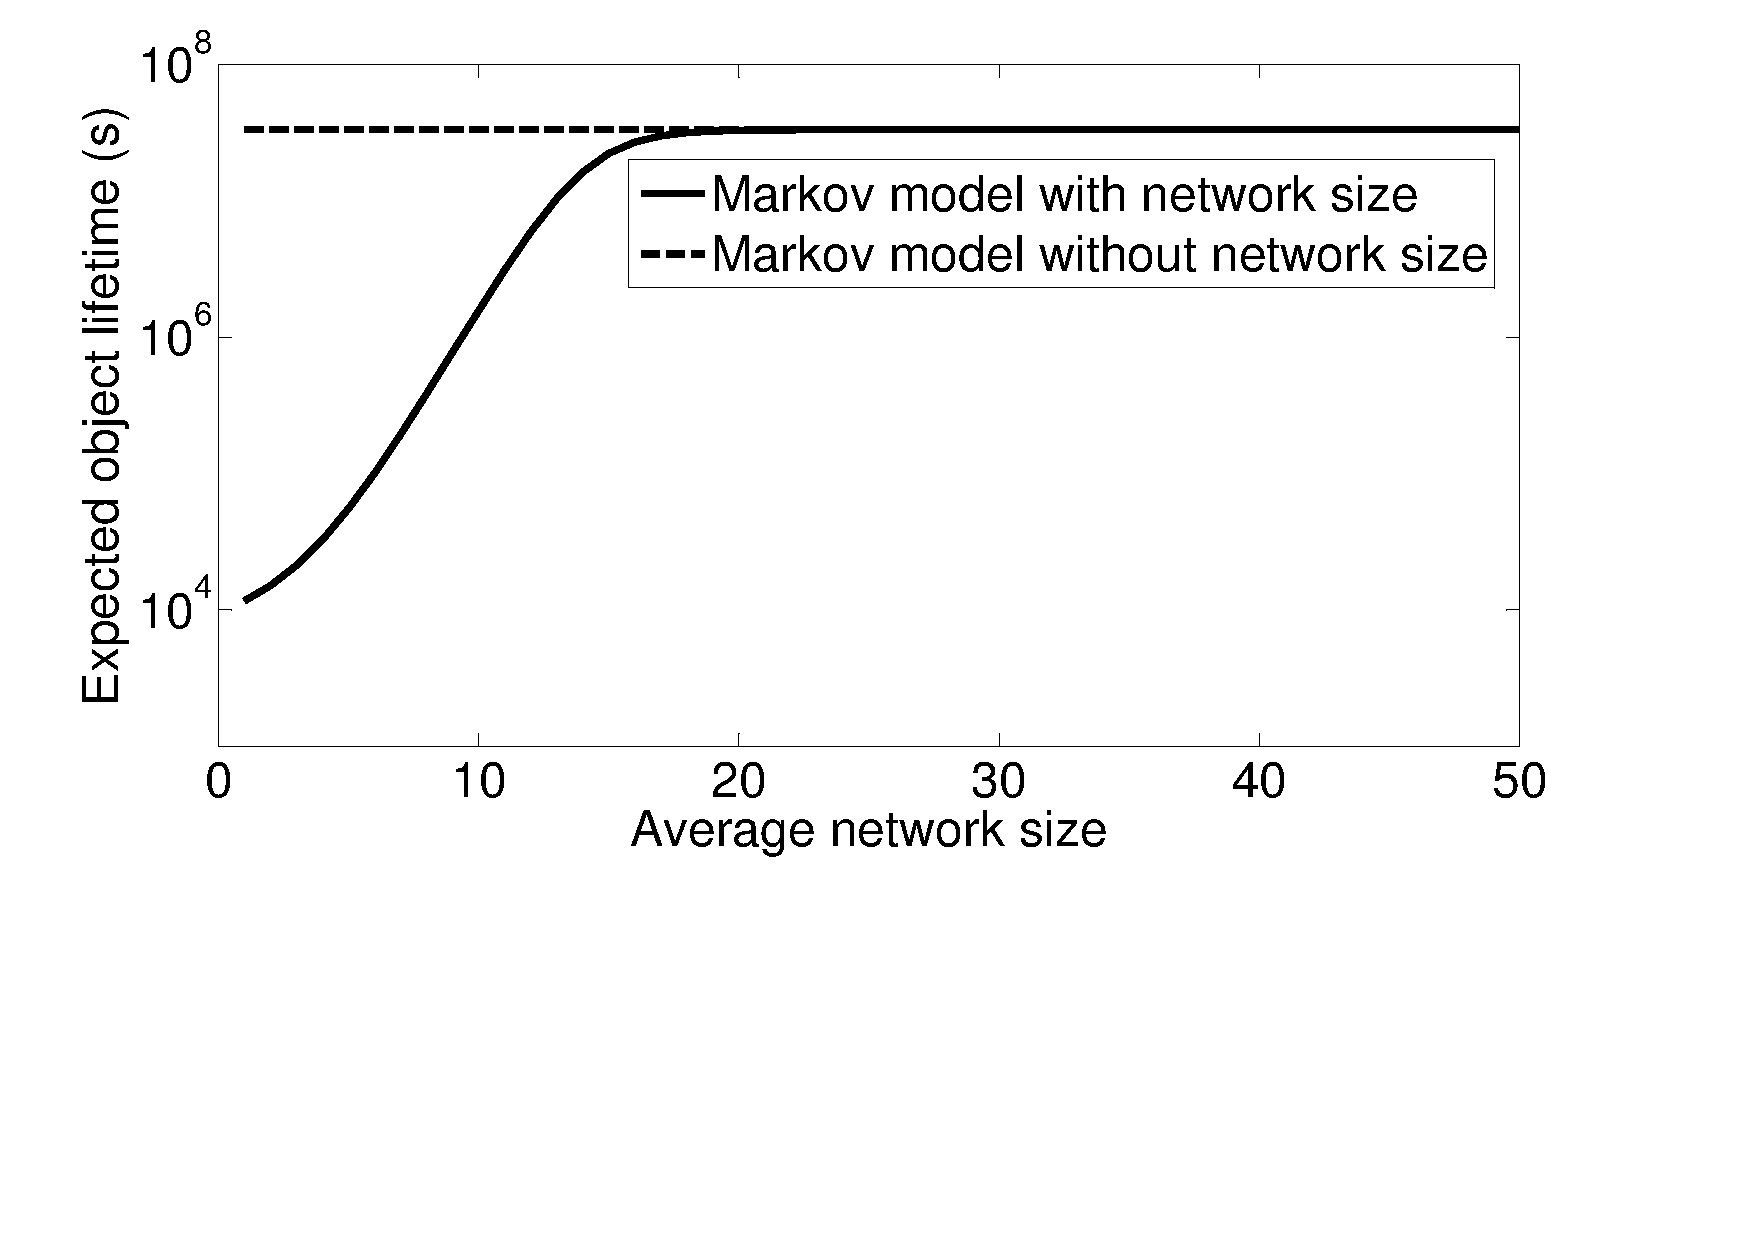
\includegraphics[clip=true, viewport=1.0cm 6.5cm 26.5cm 20.5cm, width=0.8\columnwidth]{lifetime_av_models_compare}
 \caption{Surface plot of expected object lifetimes as functions of initial and average group sizes.}
 \label{fig_lifetime_vs_other_model}
\end{figure}

Figure \ref{fig_lifetime_vs_other_model} compares the model presented in this chapter with the model of Wu, Tian and Ng that assumes object repair \cite{replication_article}. For this figure, a repair rate of $\mu = 1/180$ and a required number of replicas of $R = 10$ were used. As shown, because the model by Wu, Tian and Ng does not take average network size into account (or initial network size for that matter) it cannot predict the object lifetimes correctly for average network sizes comparable to the required number of replicas. Figure \ref{fig_lifetime_vs_other_model} verifies that the extended model presented in this chapter converges to the model that assumes an infinite network size, for sufficiently large network sizes.

\section{Comparison with Pithos simulation}
\label{simulation}

To determine practical usability of the theoretical results presented in Section \ref{results}, a comparison was performed against the Pithos simulation \cite{Pithos_mmve_2011}.

\subsection{Simulation setup}

Exponential node lifetimes were used. A single \emph{super peer} was also created and never destroyed. A single group was used, because multiple groups have different average group sizes during different simulations, which reduces the number of measurements per average group size to below statistical significance.

As with the model results generated, 10 object replicas were used. Exponential node lifetimes with 100s means were used. The shorter node lifetimes allowed for shorter object lifetimes, which allowed for more objects to be simulated in the memory available.

During a simulation run, the Pithos test application generates random objects and require these objects to be stored in the network. Every node only generated objects for 20s. This is done to limit the total number of objects present in the system to 600,000. For numbers larger than this, the simulation would run out of memory, because of the long object lifetimes when simulating cases with repair. To allow simulation of the case of long lived objects, the Pithos simulation was deployed on a ``High-Memory Quadruple Extra Large Instance'' in the Amazon EC2 cloud, which contains 68.4 GB of RAM.

Object TTLs were also set to be effectively infinite (longer than the simulation run time) to ensure that any object that is destroyed in the system is destroyed as a consequence of network churn.

For the simulation run, the overlay storage module was also turned off, since only object lifetimes in group storage were investigated. This allowed for the simulation of more objects with the memory available.

As with the previous experiments, the following configuration parameters are chosen for reasons already discussed:
%
\begin{itemize}
\item Fast group storage is used.
\item Fast group retrieval is used.
\item Simulation length of 10,000s.
\item Using the Oversim SimpleUnderlayNetwork for the physical network.
\item Object sizes of 1024 bytes.
\item Generating a store and retrieve request once every 5s.
\item All requests are for local group objects.
\end{itemize}

\subsection{No repair}

``Box and whiskers plots'' are used to compare the simulation data with the theoretical model. This allows for comparisons of mean values, but also shows how the data are distributed. In the box plot, the black striped whiskers show the minima and maxima of the data sets. The lower and upper bounds of the boxes show the 25th and 75th percentiles respectively. The horizontal lines in the boxes show the medians of the data, and the ``notches'' around the medians show the 5\% significance levels. The cross present in every box shows the simulation data mean and the solid line running through the boxes shows expected object lifetimes as predicted by the theoretical model.

\begin{figure}[htbp]
 \centering
 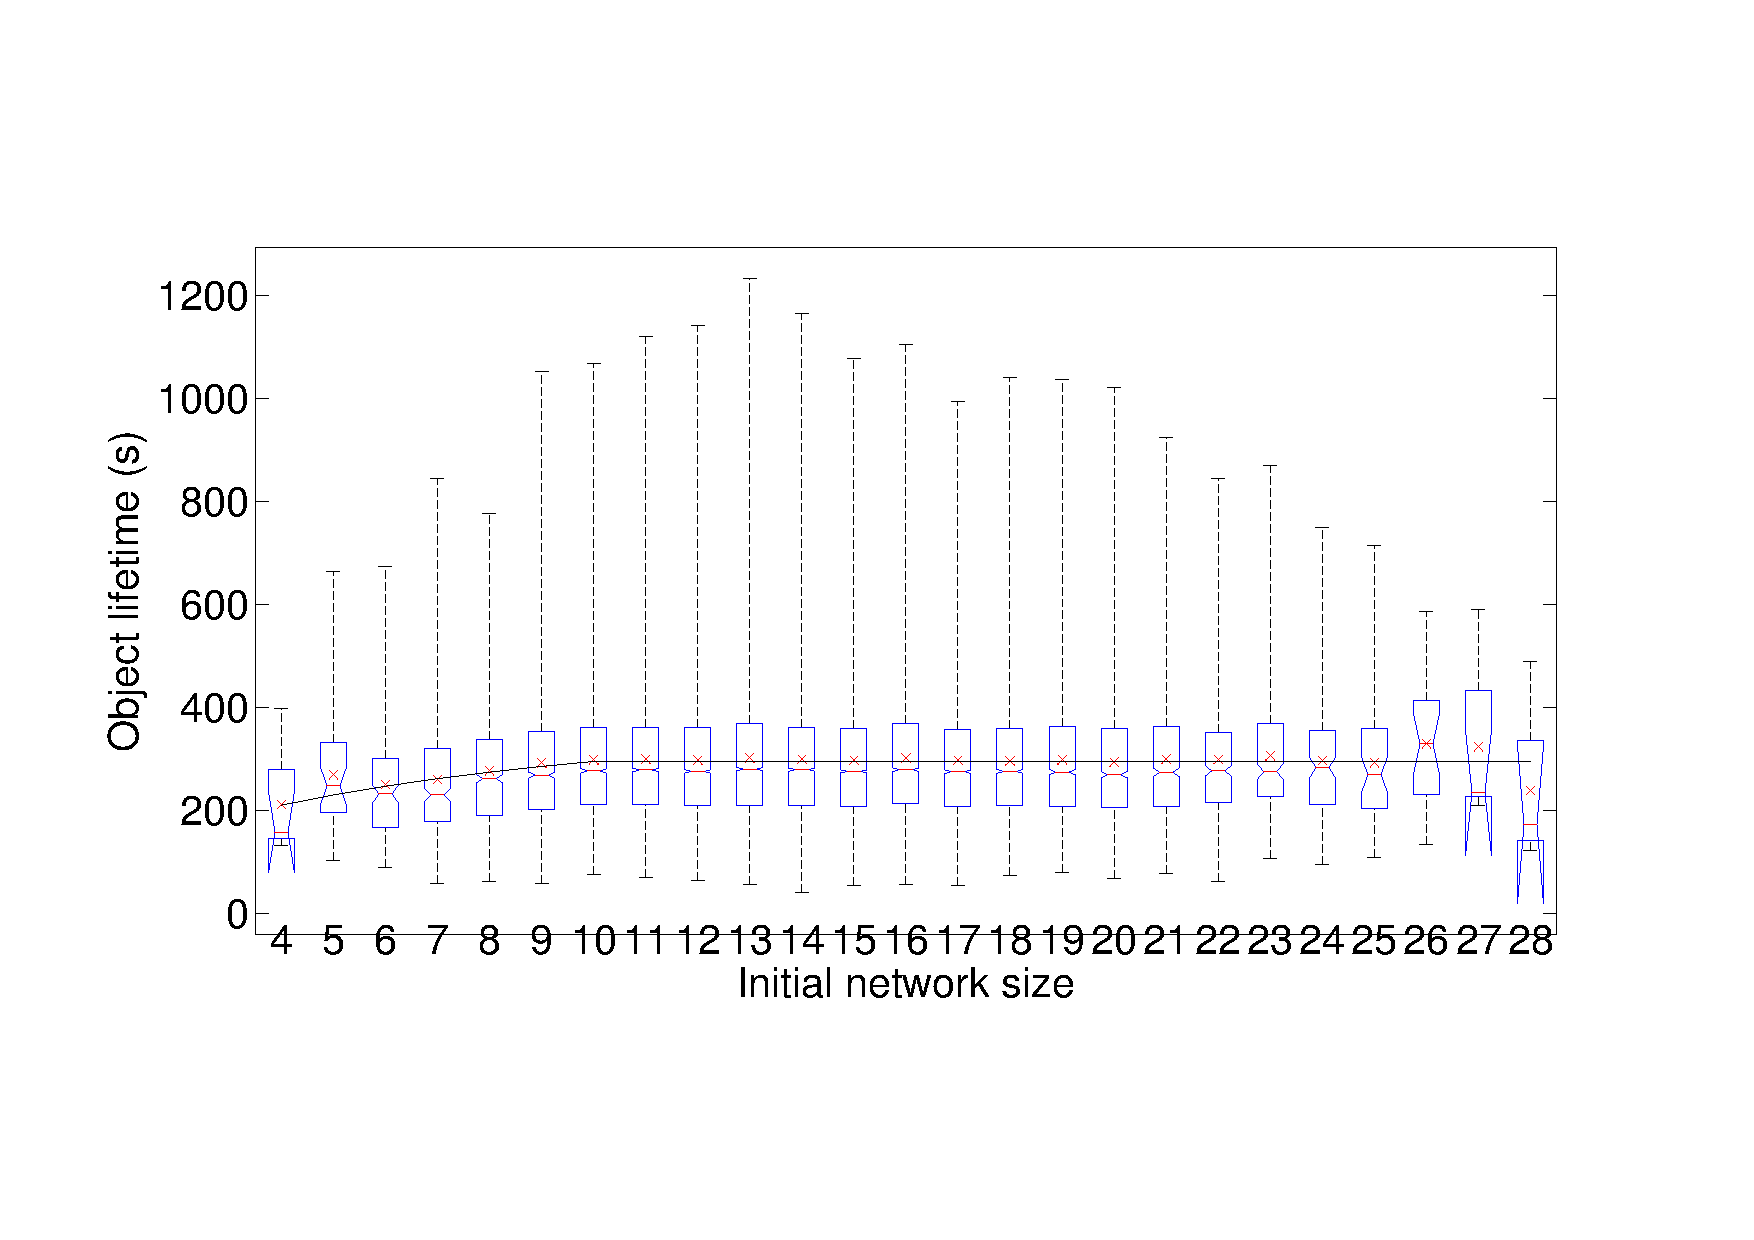
\includegraphics[clip=true, viewport=1.2cm 4.0cm 28.0cm 17cm, width=\columnwidth]{lifetime_simulation_model_none_100_30nodes}
 \caption{Comparison of object lifetime simulation results, as a box plot, with theoretical model results for no repair, node lifetimes of $100s$ and an average network size of 14 nodes.}
 \label{fig_lifetime_simulation_model_none_30_100}
\end{figure}
%
Figure \ref{fig_lifetime_simulation_model_none_30_100} compares the theoretical results to simulation results for the case where no repair is performed. Nodes have expected lifetimes of $100s$, the number of required replicas is 10 and the average network size is 14 nodes.

The expected object lifetimes as predicted by the theoretical model pass through the crosses that show the simulation data means. The mean prediction error is $4.5s$ with a standard deviation of $16.5s$. Comparing the mean prediction error to the predicted lifetime means, a mean prediction error percentage of $1.32\%$ is achieved. 

For initial network sizes on the edges of measured data, the simulation data might seem to deviate from the model data. However, in these ranges, only a few measurements could be made, instead of the thousand measurements made away from the maximum and minimum initial network size. The inaccuracy in these ranges can also be seen from the wide 5\% significance levels.

\begin{figure}[htbp]
 \centering
 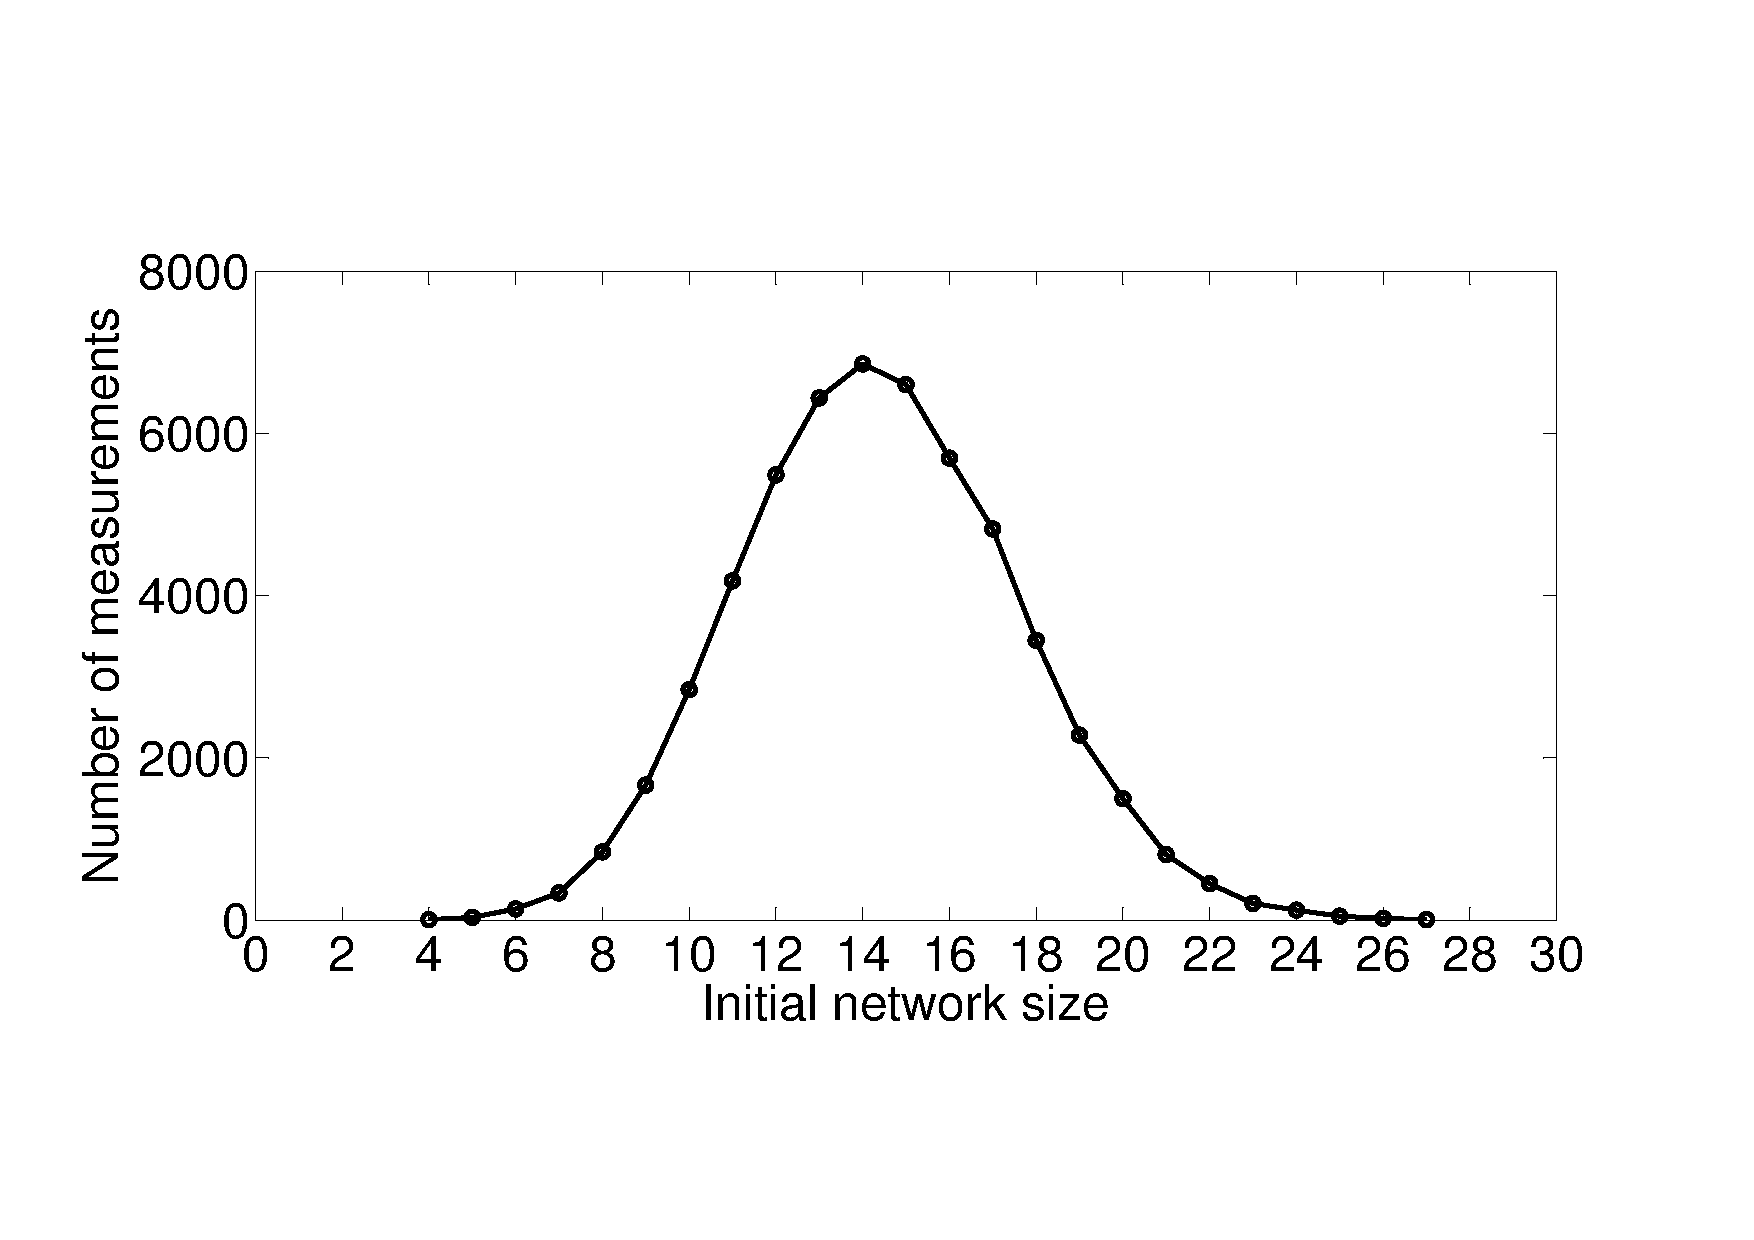
\includegraphics[clip=true, viewport=1.2cm 3.5cm 28.0cm 17cm, width=0.7\columnwidth]{lifetime_simulation_measurements_none_100_30nodes}
 \caption{Number of simulation measurements taken for the object lifetime comparison for no repair, node lifetimes of $100s$ and an average network size of 14 nodes.}
 \label{fig_lifetime_simulation_measurements_30_100}
\end{figure}
%
Figure \ref{fig_lifetime_simulation_measurements_30_100} shows the number of measurements taken for the various initial network sizes. The highest number of measurements (6855) are taken at the mean, as expected, with the number of measurements falling to 7 for initial network sizes of both 4 and 27.

\subsection{Repair time of 20s}

\begin{figure}[htbp]
 \centering
 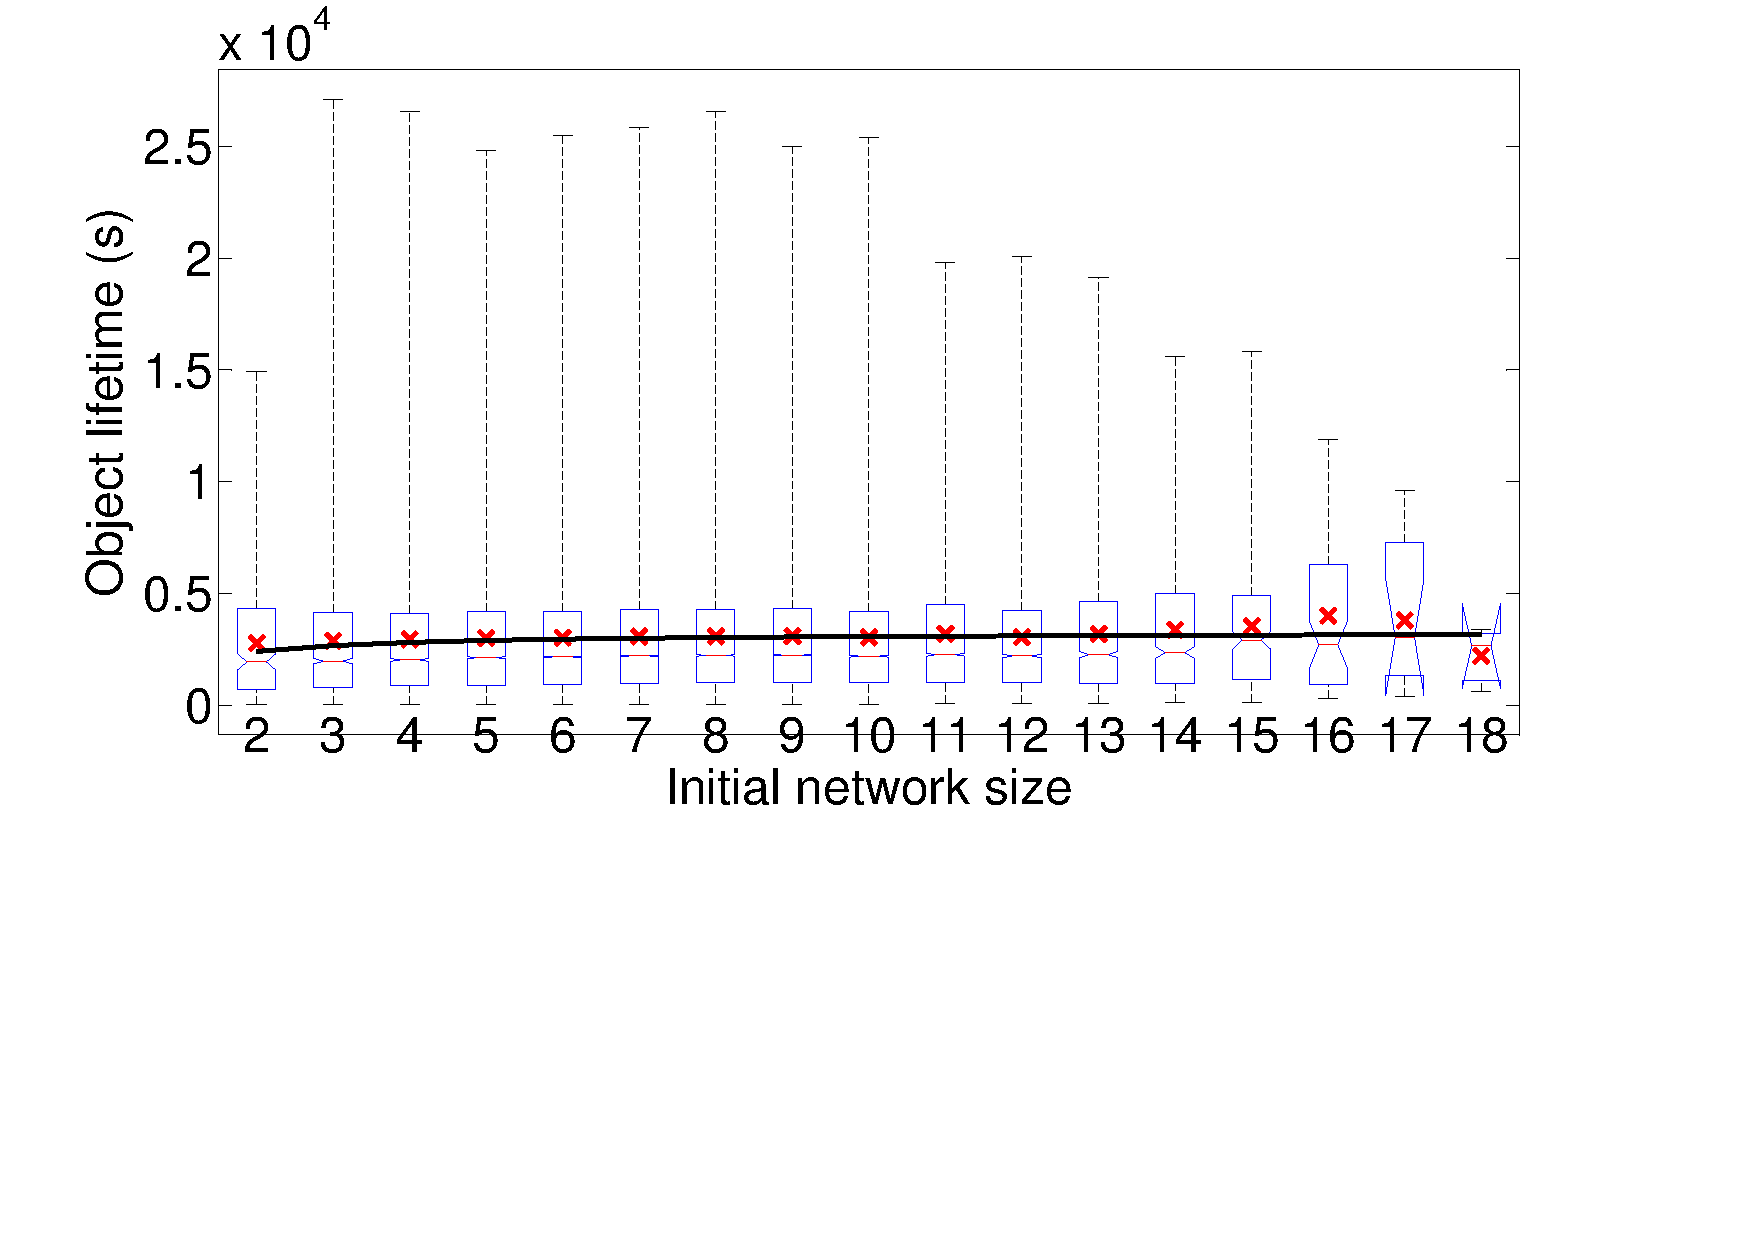
\includegraphics[clip=true, viewport=1.2cm 7.0cm 26.0cm 21cm, width=\columnwidth]{lifetime_simulation_model_20_100}
 \caption{Comparison of object lifetime simulation results, as a box plot, with theoretical model results for a repair time of $20s$, node lifetimes of $100s$ and an average network size of 7 nodes.}
 \label{fig_lifetime_simulation_model_20_100}
\end{figure}
%
Figure \ref{fig_lifetime_simulation_model_20_100} shows simulation data and theoretical model data for the same parameters as the previous figure, but for the case with $20s$ repair time. A significant increase in object lifetimes can be observed. The mean prediction error is $139.5s$ with a standard deviation of $371.3s$. Comparing the mean prediction error to the predicted lifetime means, a mean prediction error percentage of $3.18\%$ is achieved.

One issue that was encountered when comparing simulation data to model data was the imperfect repair scheme used in simulation. In the simulation, every $T_{\textrm{repair}}$ time, a repair of all objects in the system is initiated. In simulation, there is, however, a chance that the node that was chosen to repair an object leaves the network before the repair can complete. This reduces the effectiveness of the repair mechanism, reducing the effective repair rate. The percentage repair successes was measured during simulation and found to be $70\%$ exactly. All repair rates in the simulation were adjusted with this number, which successfully aligned the simulation data means with the model data means.

\subsection{Repair time of 500s}

\begin{figure}[htbp]
 \centering
 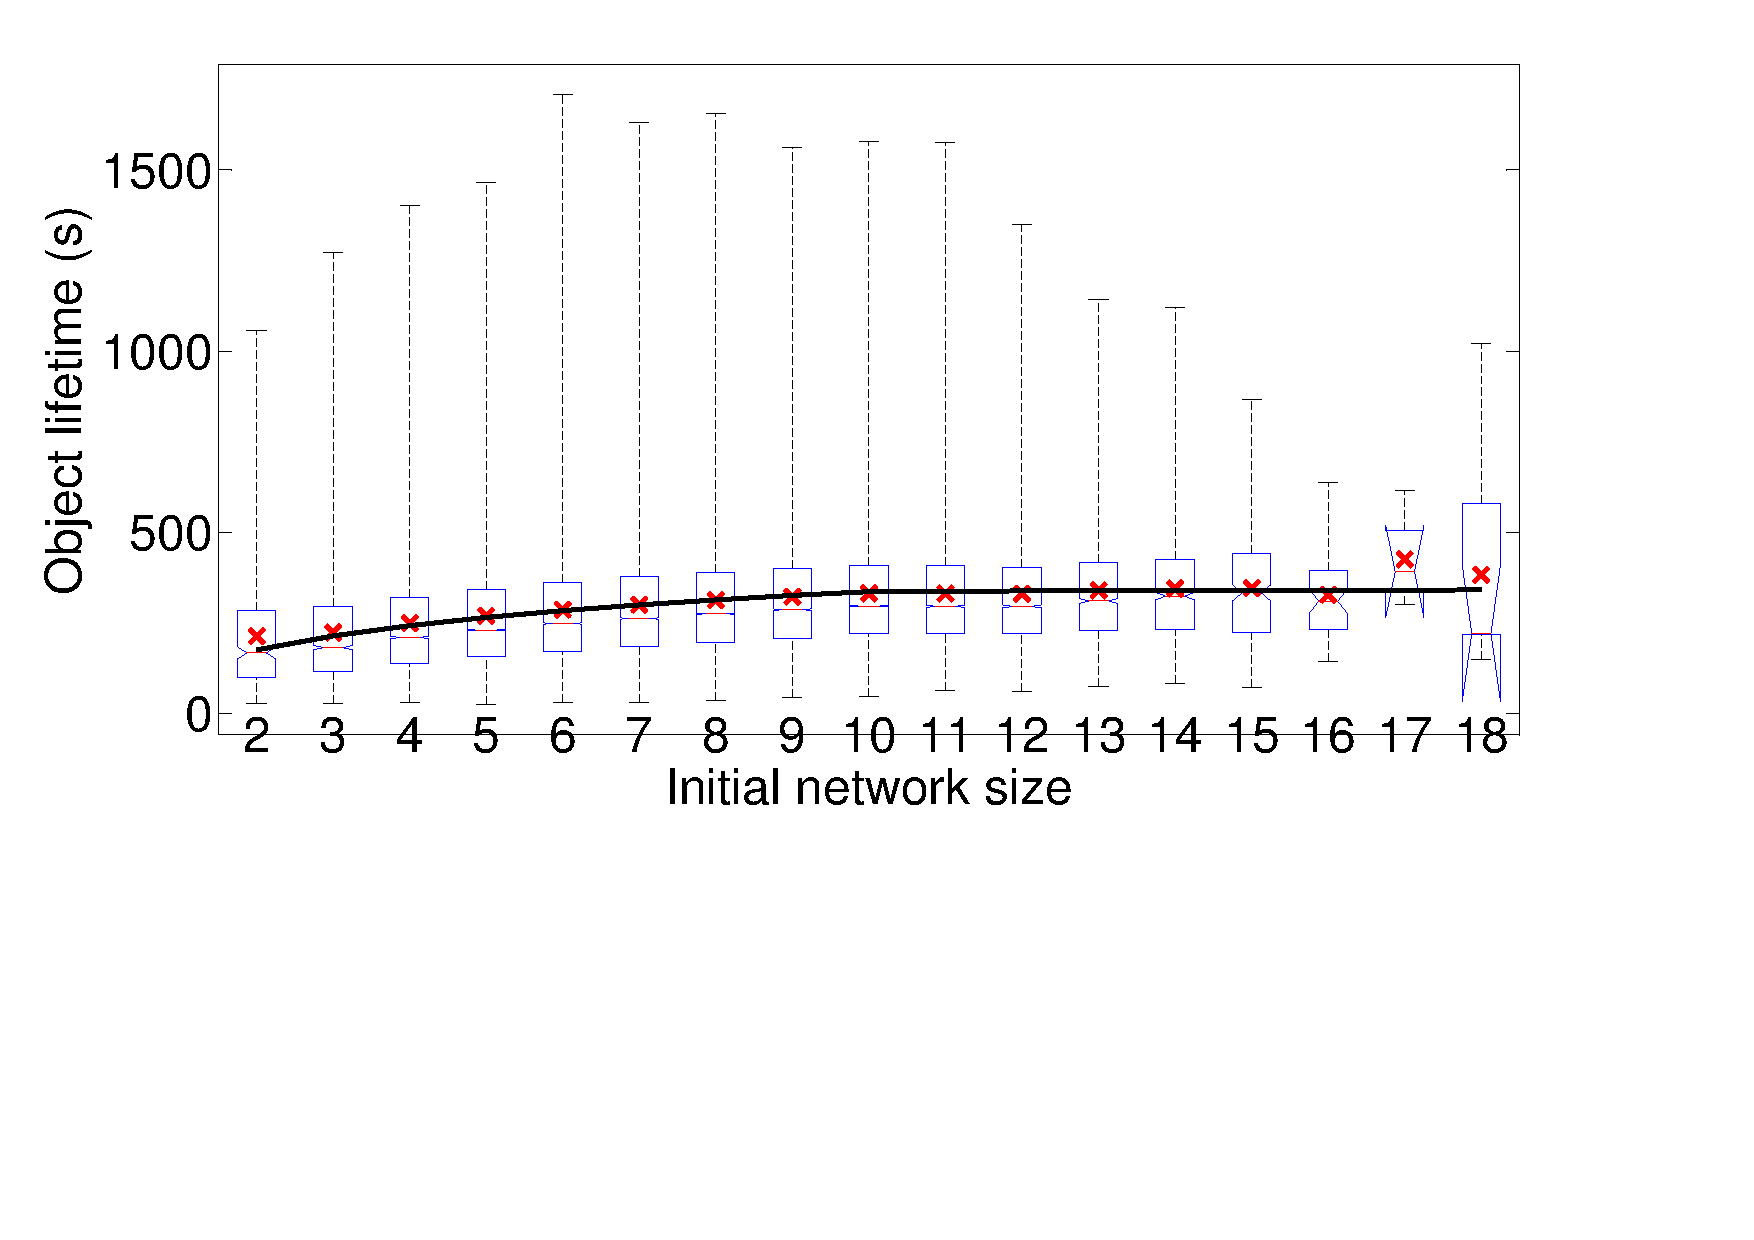
\includegraphics[clip=true, viewport=0.5cm 7cm 26.0cm 20.5cm, width=\columnwidth]{lifetime_simulation_model_500_100}
 \caption{Comparison of object lifetime simulation results, as a box plot, with theoretical model results for a repair time of $500s$, node lifetimes of $100s$ and an average network size of 7 nodes.}
 \label{fig_lifetime_simulation_model_500_100}
\end{figure}
%
Figure \ref{fig_lifetime_simulation_model_500_100} shows the simulation data and theoretical model data for the case with $500s$ repair time. The mean prediction error is $9.8s$ with a standard deviation of $23.9s$. Comparing the mean prediction error to the predicted lifetime means, a mean prediction error percentage of $3.05\%$ is achieved.

\section{Conclusion}

The Markov chain model proposed by Wu, Tian and Ng was extended to take network size into account when predicting object lifetimes. Results from the theoretical model show that when the average network size is comparable to the required number of replicas, object lifetimes are significantly decreased as is expected. The theoretical model validated the results of the model that ignores network size, when the average network size is large, compared to the required number of replicas. The model was also shown to compare well to simulation, with predicted and simulated mean object lifetimes differing on average by 3\%.

We show how to reliably predict expected object lifetimes under the assumption of finite network sizes. When it is known that the average network size is comparable to the required number of replicas, the network size should be taken into account when modelling object lifetimes in a situation with repair. The theoretical model presented here allows for the design of a distributed storage system when the various average network sizes and node lifetime distributions are known.

The theoretical model allows for the Pithos architecture to be designed with specific expected node lifetimes. It provides a guideline for the values of various parameters in the Pithos architecture, such as repair rate and required number of replicas. The expansion of the theoretical model to take into account finite networks allows for the model to accurately predict object lifetimes for small Pithos groups.

Because of the various groups that exist in Pithos, the possible range of group sizes have to be evaluated. The theoretical model will also assist in designing a system using dynamic parameters as a function of group size. 